\documentclass[11pt]{article}

    \usepackage[breakable]{tcolorbox}
    \usepackage{parskip} % Stop auto-indenting (to mimic markdown behaviour)
    
    \usepackage{iftex}
    \ifPDFTeX
    	\usepackage[T1]{fontenc}
    	\usepackage{mathpazo}
    \else
    	\usepackage{fontspec}
    \fi

    % Basic figure setup, for now with no caption control since it's done
    % automatically by Pandoc (which extracts ![](path) syntax from Markdown).
    \usepackage{graphicx}
    % Maintain compatibility with old templates. Remove in nbconvert 6.0
    \let\Oldincludegraphics\includegraphics
    % Ensure that by default, figures have no caption (until we provide a
    % proper Figure object with a Caption API and a way to capture that
    % in the conversion process - todo).
    \usepackage{caption}
    \DeclareCaptionFormat{nocaption}{}
    \captionsetup{format=nocaption,aboveskip=0pt,belowskip=0pt}

    \usepackage{float}
    \floatplacement{figure}{H} % forces figures to be placed at the correct location
    \usepackage{xcolor} % Allow colors to be defined
    \usepackage{enumerate} % Needed for markdown enumerations to work
    \usepackage{geometry} % Used to adjust the document margins
    \usepackage{amsmath} % Equations
    \usepackage{amssymb} % Equations
    \usepackage{textcomp} % defines textquotesingle
    % Hack from http://tex.stackexchange.com/a/47451/13684:
    \AtBeginDocument{%
        \def\PYZsq{\textquotesingle}% Upright quotes in Pygmentized code
    }
    \usepackage{upquote} % Upright quotes for verbatim code
    \usepackage{eurosym} % defines \euro
    \usepackage[mathletters]{ucs} % Extended unicode (utf-8) support
    \usepackage{fancyvrb} % verbatim replacement that allows latex
    \usepackage{grffile} % extends the file name processing of package graphics 
                         % to support a larger range
    \makeatletter % fix for old versions of grffile with XeLaTeX
    \@ifpackagelater{grffile}{2019/11/01}
    {
      % Do nothing on new versions
    }
    {
      \def\Gread@@xetex#1{%
        \IfFileExists{"\Gin@base".bb}%
        {\Gread@eps{\Gin@base.bb}}%
        {\Gread@@xetex@aux#1}%
      }
    }
    \makeatother
    \usepackage[Export]{adjustbox} % Used to constrain images to a maximum size
    \adjustboxset{max size={0.9\linewidth}{0.9\paperheight}}

    % The hyperref package gives us a pdf with properly built
    % internal navigation ('pdf bookmarks' for the table of contents,
    % internal cross-reference links, web links for URLs, etc.)
    \usepackage{hyperref}
    % The default LaTeX title has an obnoxious amount of whitespace. By default,
    % titling removes some of it. It also provides customization options.
    \usepackage{titling}
    \usepackage{longtable} % longtable support required by pandoc >1.10
    \usepackage{booktabs}  % table support for pandoc > 1.12.2
    \usepackage[inline]{enumitem} % IRkernel/repr support (it uses the enumerate* environment)
    \usepackage[normalem]{ulem} % ulem is needed to support strikethroughs (\sout)
                                % normalem makes italics be italics, not underlines
    \usepackage{mathrsfs}
    

    
    % Colors for the hyperref package
    \definecolor{urlcolor}{rgb}{0,.145,.698}
    \definecolor{linkcolor}{rgb}{.71,0.21,0.01}
    \definecolor{citecolor}{rgb}{.12,.54,.11}

    % ANSI colors
    \definecolor{ansi-black}{HTML}{3E424D}
    \definecolor{ansi-black-intense}{HTML}{282C36}
    \definecolor{ansi-red}{HTML}{E75C58}
    \definecolor{ansi-red-intense}{HTML}{B22B31}
    \definecolor{ansi-green}{HTML}{00A250}
    \definecolor{ansi-green-intense}{HTML}{007427}
    \definecolor{ansi-yellow}{HTML}{DDB62B}
    \definecolor{ansi-yellow-intense}{HTML}{B27D12}
    \definecolor{ansi-blue}{HTML}{208FFB}
    \definecolor{ansi-blue-intense}{HTML}{0065CA}
    \definecolor{ansi-magenta}{HTML}{D160C4}
    \definecolor{ansi-magenta-intense}{HTML}{A03196}
    \definecolor{ansi-cyan}{HTML}{60C6C8}
    \definecolor{ansi-cyan-intense}{HTML}{258F8F}
    \definecolor{ansi-white}{HTML}{C5C1B4}
    \definecolor{ansi-white-intense}{HTML}{A1A6B2}
    \definecolor{ansi-default-inverse-fg}{HTML}{FFFFFF}
    \definecolor{ansi-default-inverse-bg}{HTML}{000000}

    % common color for the border for error outputs.
    \definecolor{outerrorbackground}{HTML}{FFDFDF}

    % commands and environments needed by pandoc snippets
    % extracted from the output of `pandoc -s`
    \providecommand{\tightlist}{%
      \setlength{\itemsep}{0pt}\setlength{\parskip}{0pt}}
    \DefineVerbatimEnvironment{Highlighting}{Verbatim}{commandchars=\\\{\}}
    % Add ',fontsize=\small' for more characters per line
    \newenvironment{Shaded}{}{}
    \newcommand{\KeywordTok}[1]{\textcolor[rgb]{0.00,0.44,0.13}{\textbf{{#1}}}}
    \newcommand{\DataTypeTok}[1]{\textcolor[rgb]{0.56,0.13,0.00}{{#1}}}
    \newcommand{\DecValTok}[1]{\textcolor[rgb]{0.25,0.63,0.44}{{#1}}}
    \newcommand{\BaseNTok}[1]{\textcolor[rgb]{0.25,0.63,0.44}{{#1}}}
    \newcommand{\FloatTok}[1]{\textcolor[rgb]{0.25,0.63,0.44}{{#1}}}
    \newcommand{\CharTok}[1]{\textcolor[rgb]{0.25,0.44,0.63}{{#1}}}
    \newcommand{\StringTok}[1]{\textcolor[rgb]{0.25,0.44,0.63}{{#1}}}
    \newcommand{\CommentTok}[1]{\textcolor[rgb]{0.38,0.63,0.69}{\textit{{#1}}}}
    \newcommand{\OtherTok}[1]{\textcolor[rgb]{0.00,0.44,0.13}{{#1}}}
    \newcommand{\AlertTok}[1]{\textcolor[rgb]{1.00,0.00,0.00}{\textbf{{#1}}}}
    \newcommand{\FunctionTok}[1]{\textcolor[rgb]{0.02,0.16,0.49}{{#1}}}
    \newcommand{\RegionMarkerTok}[1]{{#1}}
    \newcommand{\ErrorTok}[1]{\textcolor[rgb]{1.00,0.00,0.00}{\textbf{{#1}}}}
    \newcommand{\NormalTok}[1]{{#1}}
    
    % Additional commands for more recent versions of Pandoc
    \newcommand{\ConstantTok}[1]{\textcolor[rgb]{0.53,0.00,0.00}{{#1}}}
    \newcommand{\SpecialCharTok}[1]{\textcolor[rgb]{0.25,0.44,0.63}{{#1}}}
    \newcommand{\VerbatimStringTok}[1]{\textcolor[rgb]{0.25,0.44,0.63}{{#1}}}
    \newcommand{\SpecialStringTok}[1]{\textcolor[rgb]{0.73,0.40,0.53}{{#1}}}
    \newcommand{\ImportTok}[1]{{#1}}
    \newcommand{\DocumentationTok}[1]{\textcolor[rgb]{0.73,0.13,0.13}{\textit{{#1}}}}
    \newcommand{\AnnotationTok}[1]{\textcolor[rgb]{0.38,0.63,0.69}{\textbf{\textit{{#1}}}}}
    \newcommand{\CommentVarTok}[1]{\textcolor[rgb]{0.38,0.63,0.69}{\textbf{\textit{{#1}}}}}
    \newcommand{\VariableTok}[1]{\textcolor[rgb]{0.10,0.09,0.49}{{#1}}}
    \newcommand{\ControlFlowTok}[1]{\textcolor[rgb]{0.00,0.44,0.13}{\textbf{{#1}}}}
    \newcommand{\OperatorTok}[1]{\textcolor[rgb]{0.40,0.40,0.40}{{#1}}}
    \newcommand{\BuiltInTok}[1]{{#1}}
    \newcommand{\ExtensionTok}[1]{{#1}}
    \newcommand{\PreprocessorTok}[1]{\textcolor[rgb]{0.74,0.48,0.00}{{#1}}}
    \newcommand{\AttributeTok}[1]{\textcolor[rgb]{0.49,0.56,0.16}{{#1}}}
    \newcommand{\InformationTok}[1]{\textcolor[rgb]{0.38,0.63,0.69}{\textbf{\textit{{#1}}}}}
    \newcommand{\WarningTok}[1]{\textcolor[rgb]{0.38,0.63,0.69}{\textbf{\textit{{#1}}}}}
    
    
    % Define a nice break command that doesn't care if a line doesn't already
    % exist.
    \def\br{\hspace*{\fill} \\* }
    % Math Jax compatibility definitions
    \def\gt{>}
    \def\lt{<}
    \let\Oldtex\TeX
    \let\Oldlatex\LaTeX
    \renewcommand{\TeX}{\textrm{\Oldtex}}
    \renewcommand{\LaTeX}{\textrm{\Oldlatex}}
    % Document parameters
    % Document title
    \title{DataVariablesAndOperations}
    
    
    
    
    
% Pygments definitions
\makeatletter
\def\PY@reset{\let\PY@it=\relax \let\PY@bf=\relax%
    \let\PY@ul=\relax \let\PY@tc=\relax%
    \let\PY@bc=\relax \let\PY@ff=\relax}
\def\PY@tok#1{\csname PY@tok@#1\endcsname}
\def\PY@toks#1+{\ifx\relax#1\empty\else%
    \PY@tok{#1}\expandafter\PY@toks\fi}
\def\PY@do#1{\PY@bc{\PY@tc{\PY@ul{%
    \PY@it{\PY@bf{\PY@ff{#1}}}}}}}
\def\PY#1#2{\PY@reset\PY@toks#1+\relax+\PY@do{#2}}

\@namedef{PY@tok@w}{\def\PY@tc##1{\textcolor[rgb]{0.73,0.73,0.73}{##1}}}
\@namedef{PY@tok@c}{\let\PY@it=\textit\def\PY@tc##1{\textcolor[rgb]{0.25,0.50,0.50}{##1}}}
\@namedef{PY@tok@cp}{\def\PY@tc##1{\textcolor[rgb]{0.74,0.48,0.00}{##1}}}
\@namedef{PY@tok@k}{\let\PY@bf=\textbf\def\PY@tc##1{\textcolor[rgb]{0.00,0.50,0.00}{##1}}}
\@namedef{PY@tok@kp}{\def\PY@tc##1{\textcolor[rgb]{0.00,0.50,0.00}{##1}}}
\@namedef{PY@tok@kt}{\def\PY@tc##1{\textcolor[rgb]{0.69,0.00,0.25}{##1}}}
\@namedef{PY@tok@o}{\def\PY@tc##1{\textcolor[rgb]{0.40,0.40,0.40}{##1}}}
\@namedef{PY@tok@ow}{\let\PY@bf=\textbf\def\PY@tc##1{\textcolor[rgb]{0.67,0.13,1.00}{##1}}}
\@namedef{PY@tok@nb}{\def\PY@tc##1{\textcolor[rgb]{0.00,0.50,0.00}{##1}}}
\@namedef{PY@tok@nf}{\def\PY@tc##1{\textcolor[rgb]{0.00,0.00,1.00}{##1}}}
\@namedef{PY@tok@nc}{\let\PY@bf=\textbf\def\PY@tc##1{\textcolor[rgb]{0.00,0.00,1.00}{##1}}}
\@namedef{PY@tok@nn}{\let\PY@bf=\textbf\def\PY@tc##1{\textcolor[rgb]{0.00,0.00,1.00}{##1}}}
\@namedef{PY@tok@ne}{\let\PY@bf=\textbf\def\PY@tc##1{\textcolor[rgb]{0.82,0.25,0.23}{##1}}}
\@namedef{PY@tok@nv}{\def\PY@tc##1{\textcolor[rgb]{0.10,0.09,0.49}{##1}}}
\@namedef{PY@tok@no}{\def\PY@tc##1{\textcolor[rgb]{0.53,0.00,0.00}{##1}}}
\@namedef{PY@tok@nl}{\def\PY@tc##1{\textcolor[rgb]{0.63,0.63,0.00}{##1}}}
\@namedef{PY@tok@ni}{\let\PY@bf=\textbf\def\PY@tc##1{\textcolor[rgb]{0.60,0.60,0.60}{##1}}}
\@namedef{PY@tok@na}{\def\PY@tc##1{\textcolor[rgb]{0.49,0.56,0.16}{##1}}}
\@namedef{PY@tok@nt}{\let\PY@bf=\textbf\def\PY@tc##1{\textcolor[rgb]{0.00,0.50,0.00}{##1}}}
\@namedef{PY@tok@nd}{\def\PY@tc##1{\textcolor[rgb]{0.67,0.13,1.00}{##1}}}
\@namedef{PY@tok@s}{\def\PY@tc##1{\textcolor[rgb]{0.73,0.13,0.13}{##1}}}
\@namedef{PY@tok@sd}{\let\PY@it=\textit\def\PY@tc##1{\textcolor[rgb]{0.73,0.13,0.13}{##1}}}
\@namedef{PY@tok@si}{\let\PY@bf=\textbf\def\PY@tc##1{\textcolor[rgb]{0.73,0.40,0.53}{##1}}}
\@namedef{PY@tok@se}{\let\PY@bf=\textbf\def\PY@tc##1{\textcolor[rgb]{0.73,0.40,0.13}{##1}}}
\@namedef{PY@tok@sr}{\def\PY@tc##1{\textcolor[rgb]{0.73,0.40,0.53}{##1}}}
\@namedef{PY@tok@ss}{\def\PY@tc##1{\textcolor[rgb]{0.10,0.09,0.49}{##1}}}
\@namedef{PY@tok@sx}{\def\PY@tc##1{\textcolor[rgb]{0.00,0.50,0.00}{##1}}}
\@namedef{PY@tok@m}{\def\PY@tc##1{\textcolor[rgb]{0.40,0.40,0.40}{##1}}}
\@namedef{PY@tok@gh}{\let\PY@bf=\textbf\def\PY@tc##1{\textcolor[rgb]{0.00,0.00,0.50}{##1}}}
\@namedef{PY@tok@gu}{\let\PY@bf=\textbf\def\PY@tc##1{\textcolor[rgb]{0.50,0.00,0.50}{##1}}}
\@namedef{PY@tok@gd}{\def\PY@tc##1{\textcolor[rgb]{0.63,0.00,0.00}{##1}}}
\@namedef{PY@tok@gi}{\def\PY@tc##1{\textcolor[rgb]{0.00,0.63,0.00}{##1}}}
\@namedef{PY@tok@gr}{\def\PY@tc##1{\textcolor[rgb]{1.00,0.00,0.00}{##1}}}
\@namedef{PY@tok@ge}{\let\PY@it=\textit}
\@namedef{PY@tok@gs}{\let\PY@bf=\textbf}
\@namedef{PY@tok@gp}{\let\PY@bf=\textbf\def\PY@tc##1{\textcolor[rgb]{0.00,0.00,0.50}{##1}}}
\@namedef{PY@tok@go}{\def\PY@tc##1{\textcolor[rgb]{0.53,0.53,0.53}{##1}}}
\@namedef{PY@tok@gt}{\def\PY@tc##1{\textcolor[rgb]{0.00,0.27,0.87}{##1}}}
\@namedef{PY@tok@err}{\def\PY@bc##1{{\setlength{\fboxsep}{\string -\fboxrule}\fcolorbox[rgb]{1.00,0.00,0.00}{1,1,1}{\strut ##1}}}}
\@namedef{PY@tok@kc}{\let\PY@bf=\textbf\def\PY@tc##1{\textcolor[rgb]{0.00,0.50,0.00}{##1}}}
\@namedef{PY@tok@kd}{\let\PY@bf=\textbf\def\PY@tc##1{\textcolor[rgb]{0.00,0.50,0.00}{##1}}}
\@namedef{PY@tok@kn}{\let\PY@bf=\textbf\def\PY@tc##1{\textcolor[rgb]{0.00,0.50,0.00}{##1}}}
\@namedef{PY@tok@kr}{\let\PY@bf=\textbf\def\PY@tc##1{\textcolor[rgb]{0.00,0.50,0.00}{##1}}}
\@namedef{PY@tok@bp}{\def\PY@tc##1{\textcolor[rgb]{0.00,0.50,0.00}{##1}}}
\@namedef{PY@tok@fm}{\def\PY@tc##1{\textcolor[rgb]{0.00,0.00,1.00}{##1}}}
\@namedef{PY@tok@vc}{\def\PY@tc##1{\textcolor[rgb]{0.10,0.09,0.49}{##1}}}
\@namedef{PY@tok@vg}{\def\PY@tc##1{\textcolor[rgb]{0.10,0.09,0.49}{##1}}}
\@namedef{PY@tok@vi}{\def\PY@tc##1{\textcolor[rgb]{0.10,0.09,0.49}{##1}}}
\@namedef{PY@tok@vm}{\def\PY@tc##1{\textcolor[rgb]{0.10,0.09,0.49}{##1}}}
\@namedef{PY@tok@sa}{\def\PY@tc##1{\textcolor[rgb]{0.73,0.13,0.13}{##1}}}
\@namedef{PY@tok@sb}{\def\PY@tc##1{\textcolor[rgb]{0.73,0.13,0.13}{##1}}}
\@namedef{PY@tok@sc}{\def\PY@tc##1{\textcolor[rgb]{0.73,0.13,0.13}{##1}}}
\@namedef{PY@tok@dl}{\def\PY@tc##1{\textcolor[rgb]{0.73,0.13,0.13}{##1}}}
\@namedef{PY@tok@s2}{\def\PY@tc##1{\textcolor[rgb]{0.73,0.13,0.13}{##1}}}
\@namedef{PY@tok@sh}{\def\PY@tc##1{\textcolor[rgb]{0.73,0.13,0.13}{##1}}}
\@namedef{PY@tok@s1}{\def\PY@tc##1{\textcolor[rgb]{0.73,0.13,0.13}{##1}}}
\@namedef{PY@tok@mb}{\def\PY@tc##1{\textcolor[rgb]{0.40,0.40,0.40}{##1}}}
\@namedef{PY@tok@mf}{\def\PY@tc##1{\textcolor[rgb]{0.40,0.40,0.40}{##1}}}
\@namedef{PY@tok@mh}{\def\PY@tc##1{\textcolor[rgb]{0.40,0.40,0.40}{##1}}}
\@namedef{PY@tok@mi}{\def\PY@tc##1{\textcolor[rgb]{0.40,0.40,0.40}{##1}}}
\@namedef{PY@tok@il}{\def\PY@tc##1{\textcolor[rgb]{0.40,0.40,0.40}{##1}}}
\@namedef{PY@tok@mo}{\def\PY@tc##1{\textcolor[rgb]{0.40,0.40,0.40}{##1}}}
\@namedef{PY@tok@ch}{\let\PY@it=\textit\def\PY@tc##1{\textcolor[rgb]{0.25,0.50,0.50}{##1}}}
\@namedef{PY@tok@cm}{\let\PY@it=\textit\def\PY@tc##1{\textcolor[rgb]{0.25,0.50,0.50}{##1}}}
\@namedef{PY@tok@cpf}{\let\PY@it=\textit\def\PY@tc##1{\textcolor[rgb]{0.25,0.50,0.50}{##1}}}
\@namedef{PY@tok@c1}{\let\PY@it=\textit\def\PY@tc##1{\textcolor[rgb]{0.25,0.50,0.50}{##1}}}
\@namedef{PY@tok@cs}{\let\PY@it=\textit\def\PY@tc##1{\textcolor[rgb]{0.25,0.50,0.50}{##1}}}

\def\PYZbs{\char`\\}
\def\PYZus{\char`\_}
\def\PYZob{\char`\{}
\def\PYZcb{\char`\}}
\def\PYZca{\char`\^}
\def\PYZam{\char`\&}
\def\PYZlt{\char`\<}
\def\PYZgt{\char`\>}
\def\PYZsh{\char`\#}
\def\PYZpc{\char`\%}
\def\PYZdl{\char`\$}
\def\PYZhy{\char`\-}
\def\PYZsq{\char`\'}
\def\PYZdq{\char`\"}
\def\PYZti{\char`\~}
% for compatibility with earlier versions
\def\PYZat{@}
\def\PYZlb{[}
\def\PYZrb{]}
\makeatother


    % For linebreaks inside Verbatim environment from package fancyvrb. 
    \makeatletter
        \newbox\Wrappedcontinuationbox 
        \newbox\Wrappedvisiblespacebox 
        \newcommand*\Wrappedvisiblespace {\textcolor{red}{\textvisiblespace}} 
        \newcommand*\Wrappedcontinuationsymbol {\textcolor{red}{\llap{\tiny$\m@th\hookrightarrow$}}} 
        \newcommand*\Wrappedcontinuationindent {3ex } 
        \newcommand*\Wrappedafterbreak {\kern\Wrappedcontinuationindent\copy\Wrappedcontinuationbox} 
        % Take advantage of the already applied Pygments mark-up to insert 
        % potential linebreaks for TeX processing. 
        %        {, <, #, %, $, ' and ": go to next line. 
        %        _, }, ^, &, >, - and ~: stay at end of broken line. 
        % Use of \textquotesingle for straight quote. 
        \newcommand*\Wrappedbreaksatspecials {% 
            \def\PYGZus{\discretionary{\char`\_}{\Wrappedafterbreak}{\char`\_}}% 
            \def\PYGZob{\discretionary{}{\Wrappedafterbreak\char`\{}{\char`\{}}% 
            \def\PYGZcb{\discretionary{\char`\}}{\Wrappedafterbreak}{\char`\}}}% 
            \def\PYGZca{\discretionary{\char`\^}{\Wrappedafterbreak}{\char`\^}}% 
            \def\PYGZam{\discretionary{\char`\&}{\Wrappedafterbreak}{\char`\&}}% 
            \def\PYGZlt{\discretionary{}{\Wrappedafterbreak\char`\<}{\char`\<}}% 
            \def\PYGZgt{\discretionary{\char`\>}{\Wrappedafterbreak}{\char`\>}}% 
            \def\PYGZsh{\discretionary{}{\Wrappedafterbreak\char`\#}{\char`\#}}% 
            \def\PYGZpc{\discretionary{}{\Wrappedafterbreak\char`\%}{\char`\%}}% 
            \def\PYGZdl{\discretionary{}{\Wrappedafterbreak\char`\$}{\char`\$}}% 
            \def\PYGZhy{\discretionary{\char`\-}{\Wrappedafterbreak}{\char`\-}}% 
            \def\PYGZsq{\discretionary{}{\Wrappedafterbreak\textquotesingle}{\textquotesingle}}% 
            \def\PYGZdq{\discretionary{}{\Wrappedafterbreak\char`\"}{\char`\"}}% 
            \def\PYGZti{\discretionary{\char`\~}{\Wrappedafterbreak}{\char`\~}}% 
        } 
        % Some characters . , ; ? ! / are not pygmentized. 
        % This macro makes them "active" and they will insert potential linebreaks 
        \newcommand*\Wrappedbreaksatpunct {% 
            \lccode`\~`\.\lowercase{\def~}{\discretionary{\hbox{\char`\.}}{\Wrappedafterbreak}{\hbox{\char`\.}}}% 
            \lccode`\~`\,\lowercase{\def~}{\discretionary{\hbox{\char`\,}}{\Wrappedafterbreak}{\hbox{\char`\,}}}% 
            \lccode`\~`\;\lowercase{\def~}{\discretionary{\hbox{\char`\;}}{\Wrappedafterbreak}{\hbox{\char`\;}}}% 
            \lccode`\~`\:\lowercase{\def~}{\discretionary{\hbox{\char`\:}}{\Wrappedafterbreak}{\hbox{\char`\:}}}% 
            \lccode`\~`\?\lowercase{\def~}{\discretionary{\hbox{\char`\?}}{\Wrappedafterbreak}{\hbox{\char`\?}}}% 
            \lccode`\~`\!\lowercase{\def~}{\discretionary{\hbox{\char`\!}}{\Wrappedafterbreak}{\hbox{\char`\!}}}% 
            \lccode`\~`\/\lowercase{\def~}{\discretionary{\hbox{\char`\/}}{\Wrappedafterbreak}{\hbox{\char`\/}}}% 
            \catcode`\.\active
            \catcode`\,\active 
            \catcode`\;\active
            \catcode`\:\active
            \catcode`\?\active
            \catcode`\!\active
            \catcode`\/\active 
            \lccode`\~`\~ 	
        }
    \makeatother

    \let\OriginalVerbatim=\Verbatim
    \makeatletter
    \renewcommand{\Verbatim}[1][1]{%
        %\parskip\z@skip
        \sbox\Wrappedcontinuationbox {\Wrappedcontinuationsymbol}%
        \sbox\Wrappedvisiblespacebox {\FV@SetupFont\Wrappedvisiblespace}%
        \def\FancyVerbFormatLine ##1{\hsize\linewidth
            \vtop{\raggedright\hyphenpenalty\z@\exhyphenpenalty\z@
                \doublehyphendemerits\z@\finalhyphendemerits\z@
                \strut ##1\strut}%
        }%
        % If the linebreak is at a space, the latter will be displayed as visible
        % space at end of first line, and a continuation symbol starts next line.
        % Stretch/shrink are however usually zero for typewriter font.
        \def\FV@Space {%
            \nobreak\hskip\z@ plus\fontdimen3\font minus\fontdimen4\font
            \discretionary{\copy\Wrappedvisiblespacebox}{\Wrappedafterbreak}
            {\kern\fontdimen2\font}%
        }%
        
        % Allow breaks at special characters using \PYG... macros.
        \Wrappedbreaksatspecials
        % Breaks at punctuation characters . , ; ? ! and / need catcode=\active 	
        \OriginalVerbatim[#1,codes*=\Wrappedbreaksatpunct]%
    }
    \makeatother

    % Exact colors from NB
    \definecolor{incolor}{HTML}{303F9F}
    \definecolor{outcolor}{HTML}{D84315}
    \definecolor{cellborder}{HTML}{CFCFCF}
    \definecolor{cellbackground}{HTML}{F7F7F7}
    
    % prompt
    \makeatletter
    \newcommand{\boxspacing}{\kern\kvtcb@left@rule\kern\kvtcb@boxsep}
    \makeatother
    \newcommand{\prompt}[4]{
        {\ttfamily\llap{{\color{#2}[#3]:\hspace{3pt}#4}}\vspace{-\baselineskip}}
    }
    

    
    % Prevent overflowing lines due to hard-to-break entities
    \sloppy 
    % Setup hyperref package
    \hypersetup{
      breaklinks=true,  % so long urls are correctly broken across lines
      colorlinks=true,
      urlcolor=urlcolor,
      linkcolor=linkcolor,
      citecolor=citecolor,
      }
    % Slightly bigger margins than the latex defaults
    
    \geometry{verbose,tmargin=1in,bmargin=1in,lmargin=1in,rmargin=1in}
    
    

\begin{document}
    
    \maketitle
    
    

    
    \hypertarget{data-variables-and-operations}{%
\section{Data, Variables and
Operations}\label{data-variables-and-operations}}

\hypertarget{topics}{%
\subsection{Topics}\label{topics}}

\begin{itemize}
\tightlist
\item
  data and values
\item
  C++ fundamental data types
\item
  digital units and number systems
\item
  variables and data assignment
\item
  keywords and operators
\item
  order of operations
\item
  operators for numbers and strings
\item
  constants
\item
  type casting
\end{itemize}

    \hypertarget{data-and-values}{%
\subsection{Data and values}\label{data-and-values}}

\begin{itemize}
\tightlist
\item
  data and values are the fundamentals to any computer language and
  program
\item
  a value is one of the fundamental things -- like a letter or a number
  -- that a program manipulates
\item
  almost all computer programs use and manipulate some data values
\end{itemize}

\hypertarget{literal-values-and-representations}{%
\subsection{Literal values and
representations}\label{literal-values-and-representations}}

\begin{itemize}
\tightlist
\item
  at a high level, we deal with two types of data values: Numbers and
  Texts
\item
  numbers can be further divided into two types:

  \begin{itemize}
  \tightlist
  \item
    Whole number literal values: 109, -234, etc.
  \item
    Floating point literal values: 123.456, -0.3555, etc.
  \end{itemize}
\item
  text is a collection of 1 or more characters (symbols, digits or
  alpahabets)

  \begin{itemize}
  \tightlist
  \item
    single character is represent using single quote ( ' )

    \begin{itemize}
    \tightlist
    \item
      char literal values: `A', `a', `\%', `1', etc.
    \end{itemize}
  \item
    2 or more characters are called string

    \begin{itemize}
    \tightlist
    \item
      represented using double quotes ( '' )
    \item
      string literal values: ``CO'', ``John Doe'', ``1100'', etc.
    \end{itemize}
  \end{itemize}
\item
  programming languages need to represent and use these data correctly
\end{itemize}

\hypertarget{c-fundamental-types}{%
\subsection{C++ fundamental types}\label{c-fundamental-types}}

\begin{itemize}
\tightlist
\item
  there are many fundamental types based on the size of the data program
  needs to store

  \begin{itemize}
  \tightlist
  \item
    most fundamental types are numeric types
  \end{itemize}
\item
  see here for all the supported types:
  https://en.cppreference.com/w/cpp/language/types
\item
  the most common types we use are:
\end{itemize}

\begin{longtable}[]{@{}llll@{}}
\toprule
Type & Description & Storage size & Value range \\
\midrule
\endhead
\textbf{void} & an empty set of values; no type & system dependent: 4 or
8 bytes & NA \\
\textbf{bool} & true or false & 1 byte or 8 bits & true or false 1 or
0 \\
\textbf{char} & one ASCII character & 1 byte or 8 bits & \(-2^7\) to
\(2^7-1\) \\
\textbf{unsigned char} & one ASCII character & 1 byte or 8 bits & 0 to
\(2^8-1\) \\
\textbf{int} & +/-ve integers & 4 bytes & \(-2^{31}\) to \(2^{31}-1\) \\
\textbf{unsigned int} & only positive integers & 4 bytes or 32 bits & 0
to \(2^{32}-1\) \\
\textbf{long} & +ve and -ve big integers & 8 bytes or 64 bits &
\(-2^{63}\) to \(2^{63}-1\) \\
\textbf{unsigned long} & positive big integers & 8 bytes or 64 bits & 0
to \(2^{64}-1\) \\
\textbf{float} & single precision floating points & 32 bits & 7 decimal
points \\
\textbf{double} & double precision floating points & 64 bits & 15
decimal points \\
\bottomrule
\end{longtable}

\begin{itemize}
\tightlist
\item
  in C++, there's no fundadamental type available to work with string
  data
\item
  two common ways to store string data:

  \begin{itemize}
  \tightlist
  \item
    use C-string or array of characters
  \item
    use basic\_string defined in
    \texttt{\textless{}string\textgreater{}} library

    \begin{itemize}
    \tightlist
    \item
      more on basic\_string:
      https://en.cppreference.com/w/cpp/string/basic\_string
    \item
      must include \texttt{\textless{}string\textgreater{}} library and
      \textbf{std} namespace
    \end{itemize}
  \end{itemize}
\item
  we'll dive into string more in depth in \textbf{Strings} chapter
\end{itemize}

\hypertarget{sizeof-operator}{%
\subsubsection{sizeof operator}\label{sizeof-operator}}

\begin{itemize}
\tightlist
\item
  one may want to know the size of memory allocated for the fundamental
  types

  \begin{itemize}
  \tightlist
  \item
    some of these types are system dependent (e.g., long is 32 bit in
    x86 and 64 bit in x64)
  \end{itemize}
\item
  \textbf{sizeof(type)} operator gives size of fundamental types in
  bytes
\item
  let's check the size of some fundamental types on my 64-bit MacBook
  Pro laptop
\end{itemize}

    \begin{tcolorbox}[breakable, size=fbox, boxrule=1pt, pad at break*=1mm,colback=cellbackground, colframe=cellborder]
\prompt{In}{incolor}{1}{\boxspacing}
\begin{Verbatim}[commandchars=\\\{\}]
\PY{k}{sizeof}\PY{p}{(}\PY{k+kt}{bool}\PY{p}{)}
\end{Verbatim}
\end{tcolorbox}

            \begin{tcolorbox}[breakable, size=fbox, boxrule=.5pt, pad at break*=1mm, opacityfill=0]
\prompt{Out}{outcolor}{1}{\boxspacing}
\begin{Verbatim}[commandchars=\\\{\}]
1
\end{Verbatim}
\end{tcolorbox}
        
    \begin{tcolorbox}[breakable, size=fbox, boxrule=1pt, pad at break*=1mm,colback=cellbackground, colframe=cellborder]
\prompt{In}{incolor}{2}{\boxspacing}
\begin{Verbatim}[commandchars=\\\{\}]
\PY{k}{sizeof}\PY{p}{(}\PY{k+kt}{char}\PY{p}{)}
\end{Verbatim}
\end{tcolorbox}

            \begin{tcolorbox}[breakable, size=fbox, boxrule=.5pt, pad at break*=1mm, opacityfill=0]
\prompt{Out}{outcolor}{2}{\boxspacing}
\begin{Verbatim}[commandchars=\\\{\}]
1
\end{Verbatim}
\end{tcolorbox}
        
    \begin{tcolorbox}[breakable, size=fbox, boxrule=1pt, pad at break*=1mm,colback=cellbackground, colframe=cellborder]
\prompt{In}{incolor}{3}{\boxspacing}
\begin{Verbatim}[commandchars=\\\{\}]
\PY{k}{sizeof}\PY{p}{(}\PY{k+kt}{int}\PY{p}{)}
\end{Verbatim}
\end{tcolorbox}

            \begin{tcolorbox}[breakable, size=fbox, boxrule=.5pt, pad at break*=1mm, opacityfill=0]
\prompt{Out}{outcolor}{3}{\boxspacing}
\begin{Verbatim}[commandchars=\\\{\}]
4
\end{Verbatim}
\end{tcolorbox}
        
    \begin{tcolorbox}[breakable, size=fbox, boxrule=1pt, pad at break*=1mm,colback=cellbackground, colframe=cellborder]
\prompt{In}{incolor}{4}{\boxspacing}
\begin{Verbatim}[commandchars=\\\{\}]
\PY{k}{sizeof}\PY{p}{(}\PY{k+kt}{long}\PY{p}{)}
\end{Verbatim}
\end{tcolorbox}

            \begin{tcolorbox}[breakable, size=fbox, boxrule=.5pt, pad at break*=1mm, opacityfill=0]
\prompt{Out}{outcolor}{4}{\boxspacing}
\begin{Verbatim}[commandchars=\\\{\}]
8
\end{Verbatim}
\end{tcolorbox}
        
    \begin{tcolorbox}[breakable, size=fbox, boxrule=1pt, pad at break*=1mm,colback=cellbackground, colframe=cellborder]
\prompt{In}{incolor}{5}{\boxspacing}
\begin{Verbatim}[commandchars=\\\{\}]
\PY{k}{sizeof}\PY{p}{(}\PY{k+kt}{float}\PY{p}{)}
\end{Verbatim}
\end{tcolorbox}

            \begin{tcolorbox}[breakable, size=fbox, boxrule=.5pt, pad at break*=1mm, opacityfill=0]
\prompt{Out}{outcolor}{5}{\boxspacing}
\begin{Verbatim}[commandchars=\\\{\}]
4
\end{Verbatim}
\end{tcolorbox}
        
    \begin{tcolorbox}[breakable, size=fbox, boxrule=1pt, pad at break*=1mm,colback=cellbackground, colframe=cellborder]
\prompt{In}{incolor}{6}{\boxspacing}
\begin{Verbatim}[commandchars=\\\{\}]
\PY{k}{sizeof}\PY{p}{(}\PY{k+kt}{double}\PY{p}{)}
\end{Verbatim}
\end{tcolorbox}

            \begin{tcolorbox}[breakable, size=fbox, boxrule=.5pt, pad at break*=1mm, opacityfill=0]
\prompt{Out}{outcolor}{6}{\boxspacing}
\begin{Verbatim}[commandchars=\\\{\}]
8
\end{Verbatim}
\end{tcolorbox}
        
    \hypertarget{units-of-digital-data}{%
\subsection{Units of digital data}\label{units-of-digital-data}}

\begin{itemize}
\tightlist
\item
  digital computers use binary number system consisting of two digits (0
  and 1)
\item
  every data and code is represented using binary values

  \begin{itemize}
  \tightlist
  \item
    hence the name binary or byte code for executable programs
  \item
    letter A is encoded as 1000001 (7 binary digits)
  \end{itemize}
\item
  humans use decimal number system with 10 digits (0 to 9)

  \begin{itemize}
  \tightlist
  \item
    we have ways to represent texts using alphabets for English language
    e.g.: Hello Bond 707!
  \item
    texts must be encoded into numbers, if we lived in the world that
    only understood numbers
  \end{itemize}
\item
  the following table shows the various units of digital data
\end{itemize}

\begin{longtable}[]{@{}ll@{}}
\toprule
Unit & Equivalent \\
\midrule
\endhead
1 bit (b) & 0 or 1 \\
1 byte (B) & 8 bits (b) \\
1 kilobyte (KB) & 1,024 B \\
1 megabyte (MB) & 1,024 KB \\
1 gigabtye (GB) & 1,024 MB \\
1 terabyte (TB) & 1,024 GB \\
1 petabyte (PB) & 1,024 TB \\
\ldots{} & \ldots{} \\
\bottomrule
\end{longtable}

    \hypertarget{number-systems}{%
\subsection{Number systems}\label{number-systems}}

\begin{itemize}
\tightlist
\item
  there are several number systems based on the base digits

  \begin{itemize}
  \tightlist
  \item
    base is number of unique digits number system uses to represent
    numbers
  \end{itemize}
\item
  binary (base 2), octal (base 8), decimal (base 10), hexadecimal (base
  16), etc.
\end{itemize}

\hypertarget{decimal-number-system}{%
\subsubsection{Decimal number system}\label{decimal-number-system}}

\begin{itemize}
\tightlist
\item
  also called Hindu-Arabic number system
\item
  most commonly used number system that uses base 10

  \begin{itemize}
  \tightlist
  \item
    has 10 digits or numerals to represent numbers: 0..9
  \item
    e.g., 1, 79, 1024, 12345, etc.
  \end{itemize}
\item
  numerals representing numbers have different place values depending on
  position:

  \begin{itemize}
  \tightlist
  \item
    ones (\(10^0\)), tens(\(10^1\)), hundreds(\(10^2\)),
    thousands(\(10^3\)), ten thousands(\(10^4\)), etc.
  \item
    e.g., 543.21 =
    \((5\times10^2)+(4\times10^1)+(3\times10^0)+(2\times10^{-1})+(1\times10^{-2})\)
  \end{itemize}
\end{itemize}

\hypertarget{number-system-conversion}{%
\subsection{Number system conversion}\label{number-system-conversion}}

\begin{itemize}
\tightlist
\item
  since computers understand only binary, everything (data, code) must
  be converted into binary
\item
  all characaters (alphabets and symbols) are given decimal codes for
  electronic communication

  \begin{itemize}
  \tightlist
  \item
    these codes are called ASCII (American Standard Code for Information
    Interchange)
  \item
    \(A \rightarrow 65; Z \rightarrow 90; a \rightarrow 97; z \rightarrow 122, * \rightarrow 42\),
    etc.
  \item
    see ASCII chart: https://en.cppreference.com/w/c/language/ascii
  \end{itemize}
\end{itemize}

\hypertarget{converting-decmial-to-binary-number}{%
\subsubsection{Converting decmial to binary
number}\label{converting-decmial-to-binary-number}}

\begin{itemize}
\tightlist
\item
  algorithm steps:

  \begin{enumerate}
  \def\labelenumi{\arabic{enumi}.}
  \tightlist
  \item
    repeteadly divide the decimal number by base \(2\) until the
    quotient becomes \(0\)

    \begin{itemize}
    \tightlist
    \item
      note remainder for each division
    \end{itemize}
  \item
    collect all the remainders in reverse order

    \begin{itemize}
    \tightlist
    \item
      the first remainder is the last (least significant) digit in
      binary
    \end{itemize}
  \end{enumerate}
\item
  example 1: what is decimal \((10)_{10}\) in binary \((?)_2\) ?

  \begin{itemize}
  \item
    step 1:

    \(\frac{10}{2}\) = quotient: \(5\), remainder: \(0\) \(\frac{5}{2}\)
    = quotient: \(2\), remainder: \(1\) \(\frac{2}{2}\) = quotient:
    \(1\), remainder: \(0\) \(\frac{1}{2}\) = quotient: \(0\),
    remainder: \(1\)
  \item
    step 2:

    \begin{itemize}
    \tightlist
    \item
      collect remainders from bottom up: \(1010\)
    \end{itemize}
  \item
    so, \((10)_{10}\) = \((1010)_2\)
  \end{itemize}
\item
  example 2: what is decimal \((13)_{10}\) in \((?)_2\) ?

  \begin{itemize}
  \item
    step 1:

    \(\frac{13}{2}\) = quotient: \(6\), remainder: \(1\) \(\frac{6}{2}\)
    = quotient \(3\), remainder: \(0\) \(\frac{3}{2}\) = quotient:
    \(1\), remainder: \(1\) \(\frac{1}{2}\) = quotient: \(0\),
    remainder: \(1\)
  \item
    step 2:

    \begin{itemize}
    \tightlist
    \item
      collect remainders from bottom up: \(1101\)
    \end{itemize}
  \item
    so, \((13)_{10}\) = \((1101)_2\)
  \end{itemize}
\end{itemize}

\hypertarget{converting-binary-to-decimal-number}{%
\subsubsection{Converting binary to decimal
number}\label{converting-binary-to-decimal-number}}

\begin{itemize}
\tightlist
\item
  once the computer does the computation in binary, it needs to convert
  the results back to decimal number system for humans to understand
\item
  algorithm steps:

  \begin{enumerate}
  \def\labelenumi{\arabic{enumi}.}
  \tightlist
  \item
    multiply each binary digit by its place value in binary
  \item
    sum all the products
  \end{enumerate}
\item
  example 1: what is binary \((1010)_2\) in decimal \((?)_{10}?\)

  \begin{itemize}
  \item
    step 1:

    \begin{itemize}
    \tightlist
    \item
      \(0\times2^0 = 0\)
    \item
      \(1\times2^1 = 2\)
    \item
      \(0\times2^2 = 0\)
    \item
      \(1\times2^3 = 8\)
    \end{itemize}
  \item
    step 2:

    \begin{itemize}
    \tightlist
    \item
      \(0 + 2 + 0 + 8 = 10\)
    \end{itemize}
  \item
    so, \((1010)_2\) = \((10)_{10}\)
  \end{itemize}
\item
  example 2: what is binary \((1101)_2\) in decimal \((?)_{10}?\)

  \begin{itemize}
  \item
    step 1:

    \begin{itemize}
    \tightlist
    \item
      \(1\times2^0 = 1\)
    \item
      \(0\times2^1 = 0\)
    \item
      \(1\times2^2 = 4\)
    \item
      \(1\times2^3 = 8\)
    \end{itemize}
  \item
    step 2:

    \begin{itemize}
    \tightlist
    \item
      \(1+0+4+8 = 13\)
    \end{itemize}
  \item
    so, \((1101)_2\) = \((13)_{10}\)
  \end{itemize}
\item
  we got the same decimal vales we started from in previous examples
\item
  food for thought: think how you'd go about writing a program to
  convert any positive decimal number into binary and vice versa!
\end{itemize}

    \hypertarget{negative-signed-integers---twos-complement}{%
\subsection{Negative (signed) integers - Two's
complement}\label{negative-signed-integers---twos-complement}}

\begin{itemize}
\tightlist
\item
  most common method of storing negative numbers on computers is a
  mathematical operation called Two's complement
\item
  Two's complement of an N-bit number is defined as its complement with
  respect to \(2^N\)

  \begin{itemize}
  \tightlist
  \item
    the sum of a number and its two's complement is \(2^N\)
  \end{itemize}
\item
  e.g.: for the 3-bit binary number \(010_2\), the two's complement is
  \(110_2\)

  \begin{itemize}
  \tightlist
  \item
    because \(010_2 + 110_2 = 1000_2 = 2^3_{10}\)
  \end{itemize}
\item
  Two's complement of N-bit number can be found by flipping each bit and
  adding one to it
\item
  e.g.~find two's complement of \(010\)

  \begin{itemize}
  \item
    Algorithm steps:

    \begin{enumerate}
    \def\labelenumi{\arabic{enumi}.}
    \tightlist
    \item
      flipped each bit; \(0\) is flipped to \(1\) and \(1\) is flipped
      to \(0\)
    \end{enumerate}

    \(010 \rightarrow 101\)

    \begin{enumerate}
    \def\labelenumi{\arabic{enumi}.}
    \setcounter{enumi}{1}
    \tightlist
    \item
      add 1 to the flipped binary
    \end{enumerate}

\begin{Shaded}
\begin{Highlighting}[]
    \ExtensionTok{101}
     \ExtensionTok{+1}
   \ExtensionTok{{-}{-}{-}{-}{-}}
    \ExtensionTok{110}
\end{Highlighting}
\end{Shaded}
  \end{itemize}
\end{itemize}

\hypertarget{example-what-is--3-decimal-in-8-bit-binary-representation}{%
\subsubsection{Example: What is -3 decimal in 8-bit binary
representation?}\label{example-what-is--3-decimal-in-8-bit-binary-representation}}

\begin{itemize}
\tightlist
\item
  convert \(3_10\) to an 8-bit binary

  \begin{itemize}
  \tightlist
  \item
    \(3_{10} \rightarrow 00000011_{2}\)
  \end{itemize}
\end{itemize}

\begin{enumerate}
\def\labelenumi{\arabic{enumi}.}
\tightlist
\item
  find Two's complement of 8-bit binary

  \begin{itemize}
  \tightlist
  \item
    \(00000011_{2} \rightarrow 11111100_{2} + 1 = 11111101_{2}\)
  \end{itemize}
\item
  Sanity check:

  \begin{itemize}
  \tightlist
  \item
    \(00000011_{2} + 11111101_{2} = 100000000_{2} = 2^8_{10}\)
  \end{itemize}
\end{enumerate}

\begin{itemize}
\tightlist
\item
  So, \(-3_{10} = 11111101_{2}\) in an 8-bit representation
\end{itemize}

    \hypertarget{exercise}{%
\subsection{Exercise}\label{exercise}}

\begin{enumerate}
\def\labelenumi{\arabic{enumi}.}
\tightlist
\item
  Convert decimal integer 7 into binary with 16 bits.
\end{enumerate}

    \begin{enumerate}
\def\labelenumi{\arabic{enumi}.}
\setcounter{enumi}{1}
\tightlist
\item
  Convert -7 decimal integer into binary with 16 bits.
\end{enumerate}

    \hypertarget{variables}{%
\subsection{Variables}\label{variables}}

\begin{itemize}
\tightlist
\item
  programs must load data values into memory to manipulate them
\item
  data may be large and used many times during the program

  \begin{itemize}
  \tightlist
  \item
    typing the data values literally all the time is not efficient and
    fun
  \item
    most importantly error prone due to typos
  \item
    you may not even know that values may be if they're read from
    standard input, files, etc.
  \end{itemize}
\item
  variables are named memory location where data can be stashed for easy
  access and manipulation
\item
  one can declared and use as many variables as necessary
\item
  C++ is statically and strongly typed programming language

  \begin{itemize}
  \tightlist
  \item
    variables are tied to their specific data types that must be
    explictly declared when declaring variables
  \end{itemize}
\end{itemize}

\hypertarget{variable-declaration}{%
\subsubsection{Variable declaration}\label{variable-declaration}}

\begin{itemize}
\tightlist
\item
  statements that create variables/identifiers to store some data values
\item
  as the name says, value of variables can vary/change over time
\item
  syntax:
\end{itemize}

\begin{Shaded}
\begin{Highlighting}[]
\NormalTok{type varName}\OperatorTok{;}
\NormalTok{type varNam1}\OperatorTok{,}\NormalTok{ varName2}\OperatorTok{,} \OperatorTok{...;} \CommentTok{//declare several variables all of the same type}
\end{Highlighting}
\end{Shaded}

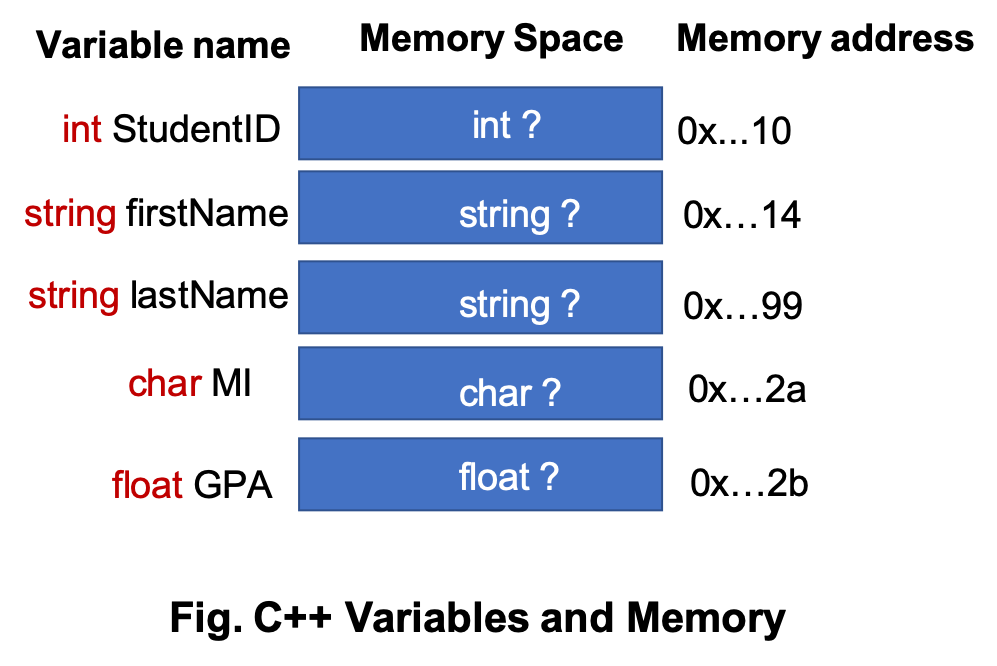
\includegraphics{resources/VariablesAndMemory.png}

\hypertarget{rules-for-creating-variables}{%
\subsubsection{Rules for creating
variables}\label{rules-for-creating-variables}}

\begin{itemize}
\tightlist
\item
  variable names are case sensitive
\item
  must declare variables before they can be used
\item
  can't define variable with the same name more than once
\item
  can't use keywords as variable names
\item
  data stored must match the type of variable
\item
  variable names can't contain symbols (white spaces, \#, \&, etc.)
  except for \_ and \$ (underscore and dollar)
\item
  variable names can contain digits but can't start with a digit
\item
  variable names can start with only alphabets (lower or upper) and \_
  symbol
\end{itemize}

\hypertarget{best-practices}{%
\subsubsection{Best practices}\label{best-practices}}

\begin{itemize}
\tightlist
\item
  use descriptive and meaningful but concise name

  \begin{itemize}
  \tightlist
  \item
    one should know quickly what data you're storing
  \end{itemize}
\item
  use lowercase; camelCase or ( \_ underscore ) to combine multiple
  words
\end{itemize}

\hypertarget{c-keywords}{%
\subsubsection{C++ keywords}\label{c-keywords}}

\begin{itemize}
\tightlist
\item
  keywords are reserved names and words that have specific purpose in
  C++

  \begin{itemize}
  \tightlist
  \item
    they can only be used what they're intended for
  \end{itemize}
\item
  e.g., char, int, unsigned, signed, float, double, bool, if, for,
  while, return, struct, class, operator, try, etc.
\item
  all C++ keywords are listed here:
  https://en.cppreference.com/w/cpp/keyword
\end{itemize}

    \begin{tcolorbox}[breakable, size=fbox, boxrule=1pt, pad at break*=1mm,colback=cellbackground, colframe=cellborder]
\prompt{In}{incolor}{7}{\boxspacing}
\begin{Verbatim}[commandchars=\\\{\}]
\PY{c+c1}{// examples of variable declaration}
\PY{k+kt}{bool} \PY{n}{done}\PY{p}{;}
\PY{k+kt}{char} \PY{n}{middleInitial}\PY{p}{;}
\PY{k+kt}{char} \PY{n}{middleinitial}\PY{p}{;} \PY{c+c1}{// hard to read all lowercase name}
\PY{k+kt}{int} \PY{n}{temperature}\PY{p}{;}
\PY{k+kt}{unsigned} \PY{k+kt}{int} \PY{n}{age}\PY{p}{;}
\PY{k+kt}{long} \PY{n}{richest\PYZus{}persons\PYZus{}networth}\PY{p}{;}
\PY{k+kt}{float} \PY{n}{interestRate}\PY{p}{;}
\PY{k+kt}{float} \PY{n}{length}\PY{p}{;}
\PY{k+kt}{float} \PY{n}{width}\PY{p}{;}
\PY{k+kt}{double} \PY{n}{space\PYZus{}shuttle\PYZus{}velocity}\PY{p}{;}
\end{Verbatim}
\end{tcolorbox}

    \begin{tcolorbox}[breakable, size=fbox, boxrule=1pt, pad at break*=1mm,colback=cellbackground, colframe=cellborder]
\prompt{In}{incolor}{8}{\boxspacing}
\begin{Verbatim}[commandchars=\\\{\}]
\PY{c+c1}{// TODO:}
\PY{c+c1}{// Declare 10 variables of atleast 5 different types}
\end{Verbatim}
\end{tcolorbox}

    \hypertarget{string-variables}{%
\subsubsection{String variables}\label{string-variables}}

\begin{itemize}
\tightlist
\item
  declare variables that store string data

  \begin{itemize}
  \tightlist
  \item
    1 or more string of characters
  \end{itemize}
\item
  an easy way to use string is by using C++ advanced type defined in
  \texttt{\textless{}string\textgreater{}} header file
\item
  must include \texttt{\textless{}string\textgreater{}} header file or
  library to use string type
\item
  must also use \textbf{std} namespace
\item
  strings are represented using a pair of double quotes (``string'')
\item
  more on string type is covered in \textbf{Strings} chapter
\item
  the following are some examples of string variables
\end{itemize}

    \begin{tcolorbox}[breakable, size=fbox, boxrule=1pt, pad at break*=1mm,colback=cellbackground, colframe=cellborder]
\prompt{In}{incolor}{9}{\boxspacing}
\begin{Verbatim}[commandchars=\\\{\}]
\PY{c+c1}{// string variables}
\PY{c+cp}{\PYZsh{}}\PY{c+cp}{include} \PY{c+cpf}{\PYZlt{}string\PYZgt{}}

\PY{k}{using} \PY{k}{namespace} \PY{n+nn}{std}\PY{p}{;}

\PY{n}{string} \PY{n}{fullName}\PY{p}{;}
\PY{n}{string} \PY{n}{firstName}\PY{p}{;}
\PY{n}{string} \PY{n}{address1}\PY{p}{;}
\PY{n}{string} \PY{n}{country}\PY{p}{;}
\PY{n}{string} \PY{n}{state\PYZus{}name}\PY{p}{;}
\PY{n}{std}\PY{o}{:}\PY{o}{:}\PY{n}{string} \PY{n}{state\PYZus{}code}\PY{p}{;} \PY{c+c1}{// :: name resolution operator}
\end{Verbatim}
\end{tcolorbox}

    \begin{tcolorbox}[breakable, size=fbox, boxrule=1pt, pad at break*=1mm,colback=cellbackground, colframe=cellborder]
\prompt{In}{incolor}{10}{\boxspacing}
\begin{Verbatim}[commandchars=\\\{\}]
\PY{c+c1}{// TODO:}
\PY{c+c1}{// Declare 5 string variables}
\end{Verbatim}
\end{tcolorbox}

    \hypertarget{assignment-operator}{%
\subsection{Assignment operator ( = )}\label{assignment-operator}}

\begin{itemize}
\tightlist
\item
  once variables are declared, data can be stored using assignment
  operator, \$ = \$
\item
  \textbf{assignment statements} have the following syntax:
\end{itemize}

\begin{Shaded}
\begin{Highlighting}[]
\NormalTok{varName }\OperatorTok{=}\NormalTok{ value}\OperatorTok{;}
\end{Highlighting}
\end{Shaded}

\begin{itemize}
\tightlist
\item
  since C++ is a strongly typed language, the type of value must match
  the type of variable

  \begin{itemize}
  \tightlist
  \item
    strongly typed languages enforces type safety and matching during
    the compile time
  \end{itemize}
\end{itemize}

    \begin{tcolorbox}[breakable, size=fbox, boxrule=1pt, pad at break*=1mm,colback=cellbackground, colframe=cellborder]
\prompt{In}{incolor}{11}{\boxspacing}
\begin{Verbatim}[commandchars=\\\{\}]
\PY{c+c1}{// assignment examples}
\PY{n}{done} \PY{o}{=} \PY{n+nb}{false}\PY{p}{;}
\PY{n}{middleInitial} \PY{o}{=} \PY{l+s+sc}{\PYZsq{}}\PY{l+s+sc}{J}\PY{l+s+sc}{\PYZsq{}}\PY{p}{;} \PY{c+c1}{// character is represent using single quote}
\PY{n}{middleinitial} \PY{o}{=} \PY{l+s+sc}{\PYZsq{}}\PY{l+s+sc}{Q}\PY{l+s+sc}{\PYZsq{}}\PY{p}{;}
\PY{n}{temperature} \PY{o}{=} \PY{l+m+mi}{73}\PY{p}{;}
\PY{n}{age} \PY{o}{=} \PY{l+m+mi}{45}\PY{p}{;}
\PY{n}{richest\PYZus{}persons\PYZus{}networth} \PY{o}{=} \PY{l+m+mi}{120000000000}\PY{p}{;} \PY{c+c1}{// 120 billion}
\PY{n}{interestRate} \PY{o}{=} \PY{l+m+mf}{4.5}\PY{p}{;}
\PY{n}{length} \PY{o}{=} \PY{l+m+mf}{10.5}\PY{p}{;}
\PY{n}{width} \PY{o}{=} \PY{l+m+mf}{99.99f}\PY{p}{;} \PY{c+c1}{// number can end with f to represent as float}
\PY{n}{space\PYZus{}shuttle\PYZus{}velocity} \PY{o}{=} \PY{l+m+mf}{950.1234567891234567}\PY{p}{;} \PY{c+c1}{// 16 decimal points}
\end{Verbatim}
\end{tcolorbox}

            \begin{tcolorbox}[breakable, size=fbox, boxrule=.5pt, pad at break*=1mm, opacityfill=0]
\prompt{Out}{outcolor}{11}{\boxspacing}
\begin{Verbatim}[commandchars=\\\{\}]
950.123
\end{Verbatim}
\end{tcolorbox}
        
    \begin{tcolorbox}[breakable, size=fbox, boxrule=1pt, pad at break*=1mm,colback=cellbackground, colframe=cellborder]
\prompt{In}{incolor}{12}{\boxspacing}
\begin{Verbatim}[commandchars=\\\{\}]
\PY{c+c1}{// string assignment examples}
\PY{n}{fullName} \PY{o}{=} \PY{l+s}{\PYZdq{}}\PY{l+s}{John Doe}\PY{l+s}{\PYZdq{}}\PY{p}{;}
\PY{n}{firstName} \PY{o}{=} \PY{l+s}{\PYZdq{}}\PY{l+s}{John}\PY{l+s}{\PYZdq{}}\PY{p}{;}
\PY{n}{address1} \PY{o}{=} \PY{l+s}{\PYZdq{}}\PY{l+s}{1100 North Avenue}\PY{l+s}{\PYZdq{}}\PY{p}{;} \PY{c+c1}{// number as string}
\PY{n}{country} \PY{o}{=} \PY{l+s}{\PYZdq{}}\PY{l+s}{USA}\PY{l+s}{\PYZdq{}}\PY{p}{;}
\PY{n}{state\PYZus{}name} \PY{o}{=} \PY{l+s}{\PYZdq{}}\PY{l+s}{Colorado}\PY{l+s}{\PYZdq{}}\PY{p}{;}
\PY{n}{state\PYZus{}code} \PY{o}{=} \PY{l+s}{\PYZdq{}}\PY{l+s}{CO}\PY{l+s}{\PYZdq{}}\PY{p}{;}
\end{Verbatim}
\end{tcolorbox}

    \begin{tcolorbox}[breakable, size=fbox, boxrule=1pt, pad at break*=1mm,colback=cellbackground, colframe=cellborder]
\prompt{In}{incolor}{13}{\boxspacing}
\begin{Verbatim}[commandchars=\\\{\}]
\PY{c+c1}{// TODO: assign different values to variables defined above}
\end{Verbatim}
\end{tcolorbox}

    \hypertarget{variable-declartion-and-initialization}{%
\subsubsection{Variable declartion and
initialization}\label{variable-declartion-and-initialization}}

\begin{itemize}
\tightlist
\item
  variables can be declared with initial value at the time of
  construction
\item
  if you know what value a variable should start with; this saves you
  typing
\item
  often times its the best practice to initialize variable with default
  value
\item
  several ways to initialize variables:
  https://en.cppreference.com/w/cpp/language/initialization
\item
  two common ways:

  \begin{enumerate}
  \def\labelenumi{\arabic{enumi}.}
  \tightlist
  \item
    Copy initialization (using \texttt{=} operator)
  \item
    Value initialization (using \texttt{\{\ \}} curley braces)

    \begin{itemize}
    \tightlist
    \item
      also called uniform initialization
    \item
      useful in initializing advanced types such as arrays, objects,
      etc.
    \end{itemize}
  \end{enumerate}
\end{itemize}

    \begin{tcolorbox}[breakable, size=fbox, boxrule=1pt, pad at break*=1mm,colback=cellbackground, colframe=cellborder]
\prompt{In}{incolor}{14}{\boxspacing}
\begin{Verbatim}[commandchars=\\\{\}]
\PY{c+c1}{// Copy initialization}
\PY{k+kt}{float} \PY{n}{price} \PY{o}{=} \PY{l+m+mf}{2.99f}\PY{p}{;}
\PY{k+kt}{char} \PY{n}{MI} \PY{o}{=} \PY{l+s+sc}{\PYZsq{}}\PY{l+s+sc}{B}\PY{l+s+sc}{\PYZsq{}}\PY{p}{;} \PY{c+c1}{//middle initial}
\PY{n}{string} \PY{n}{school\PYZus{}name} \PY{o}{=} \PY{l+s}{\PYZdq{}}\PY{l+s}{Grand Junction High}\PY{l+s}{\PYZdq{}}\PY{p}{;}
\end{Verbatim}
\end{tcolorbox}

    \begin{tcolorbox}[breakable, size=fbox, boxrule=1pt, pad at break*=1mm,colback=cellbackground, colframe=cellborder]
\prompt{In}{incolor}{15}{\boxspacing}
\begin{Verbatim}[commandchars=\\\{\}]
\PY{c+c1}{// Value/uniform initialization}
\PY{k+kt}{char} \PY{n}{some\PYZus{}letter}\PY{p}{\PYZob{}}\PY{l+s+sc}{\PYZsq{}}\PY{l+s+sc}{U}\PY{l+s+sc}{\PYZsq{}}\PY{p}{\PYZcb{}}\PY{p}{;}
\PY{k+kt}{int} \PY{n}{some\PYZus{}length}\PY{p}{\PYZob{}}\PY{l+m+mi}{100}\PY{p}{\PYZcb{}}\PY{p}{;}
\PY{k+kt}{float} \PY{n}{some\PYZus{}float}\PY{p}{\PYZob{}}\PY{l+m+mf}{200.99}\PY{p}{\PYZcb{}}\PY{p}{;}
\PY{n}{string} \PY{n}{some\PYZus{}string} \PY{o}{=} \PY{p}{\PYZob{}}\PY{l+s}{\PYZdq{}}\PY{l+s}{Hello World!}\PY{l+s}{\PYZdq{}}\PY{p}{\PYZcb{}}\PY{p}{;} \PY{c+c1}{// can also combine the two!}
\end{Verbatim}
\end{tcolorbox}

    \hypertarget{variables-value-can-be-changed}{%
\subsubsection{Variable's value can be
changed}\label{variables-value-can-be-changed}}

\begin{itemize}
\tightlist
\item
  variable's value can vary through out the program

  \begin{itemize}
  \tightlist
  \item
    hence the name variable
  \end{itemize}
\item
  however, type of the value must be same as the type of the variable
  declared
\item
  C++ is a strongly and statically typed programming language!
\end{itemize}

    \begin{tcolorbox}[breakable, size=fbox, boxrule=1pt, pad at break*=1mm,colback=cellbackground, colframe=cellborder]
\prompt{In}{incolor}{16}{\boxspacing}
\begin{Verbatim}[commandchars=\\\{\}]
\PY{n}{price} \PY{o}{=} \PY{l+m+mf}{3.99}\PY{p}{;}
\PY{n}{price} \PY{o}{=} \PY{l+m+mf}{1.99}\PY{p}{;}
\PY{n}{MI} \PY{o}{=} \PY{l+s+sc}{\PYZsq{}}\PY{l+s+sc}{Q}\PY{l+s+sc}{\PYZsq{}}\PY{p}{;}
\PY{n}{school\PYZus{}name} \PY{o}{=} \PY{l+s}{\PYZdq{}}\PY{l+s}{Fruita Monument High}\PY{l+s}{\PYZdq{}}\PY{p}{;}
\PY{n}{some\PYZus{}string} \PY{o}{=} \PY{l+s}{\PYZdq{}}\PY{l+s}{Goodbye, World!}\PY{l+s}{\PYZdq{}}\PY{p}{;}
\end{Verbatim}
\end{tcolorbox}

    \begin{tcolorbox}[breakable, size=fbox, boxrule=1pt, pad at break*=1mm,colback=cellbackground, colframe=cellborder]
\prompt{In}{incolor}{17}{\boxspacing}
\begin{Verbatim}[commandchars=\\\{\}]
\PY{n}{price} \PY{o}{=} \PY{l+s}{\PYZdq{}}\PY{l+s}{4.99}\PY{l+s}{\PYZdq{}}\PY{p}{;} \PY{c+c1}{// is this valid?}
\end{Verbatim}
\end{tcolorbox}

    \begin{Verbatim}[commandchars=\\\{\}]
\textbf{input\_line\_34:2:10: }\textcolor{ansi-red-intense}{\textbf{error: }}\textbf{assigning to 'float' from
incompatible type 'const char [5]'}
 price = "4.99";
\textcolor{ansi-green-intense}{\textbf{         \^{}\textasciitilde{}\textasciitilde{}\textasciitilde{}\textasciitilde{}\textasciitilde{}
}}
    \end{Verbatim}

    \begin{Verbatim}[commandchars=\\\{\}, frame=single, framerule=2mm, rulecolor=\color{outerrorbackground}]
Interpreter Error: 
    \end{Verbatim}

    \hypertarget{auto-type}{%
\subsubsection{auto type}\label{auto-type}}

\begin{itemize}
\tightlist
\item
  if variable is declared and initialized in one statement, you can use
  \textbf{auto} keyword to let compiler determine type of variable based
  on the value it's initialized with
\end{itemize}

    \begin{tcolorbox}[breakable, size=fbox, boxrule=1pt, pad at break*=1mm,colback=cellbackground, colframe=cellborder]
\prompt{In}{incolor}{18}{\boxspacing}
\begin{Verbatim}[commandchars=\\\{\}]
\PY{k}{auto} \PY{n}{var1} \PY{o}{=} \PY{l+m+mi}{10}\PY{p}{;} \PY{c+c1}{// integer}
\PY{k}{auto} \PY{n}{var2} \PY{o}{=} \PY{l+m+mf}{19.99f}\PY{p}{;} \PY{c+c1}{// float}
\PY{k}{auto} \PY{n}{var3} \PY{o}{=} \PY{l+m+mf}{99.245}\PY{p}{;} \PY{c+c1}{// double}
\PY{k}{auto} \PY{n}{var4} \PY{o}{=} \PY{l+s+sc}{\PYZsq{}}\PY{l+s+sc}{@}\PY{l+s+sc}{\PYZsq{}}\PY{p}{;} \PY{c+c1}{// char}
\end{Verbatim}
\end{tcolorbox}

    \begin{tcolorbox}[breakable, size=fbox, boxrule=1pt, pad at break*=1mm,colback=cellbackground, colframe=cellborder]
\prompt{In}{incolor}{19}{\boxspacing}
\begin{Verbatim}[commandchars=\\\{\}]
\PY{c+c1}{// char * (pointer) type and not string type}
\PY{k}{auto} \PY{n}{full\PYZus{}name} \PY{o}{=} \PY{l+s}{\PYZdq{}}\PY{l+s}{John Doe}\PY{l+s}{\PYZdq{}}\PY{p}{;}
\end{Verbatim}
\end{tcolorbox}

    \begin{tcolorbox}[breakable, size=fbox, boxrule=1pt, pad at break*=1mm,colback=cellbackground, colframe=cellborder]
\prompt{In}{incolor}{20}{\boxspacing}
\begin{Verbatim}[commandchars=\\\{\}]
\PY{c+c1}{// can automatically declare string type}
\PY{c+cp}{\PYZsh{}}\PY{c+cp}{include} \PY{c+cpf}{\PYZlt{}string\PYZgt{}}
\PY{k}{using} \PY{k}{namespace} \PY{n+nn}{std}\PY{p}{;}

\PY{k}{auto} \PY{n}{full\PYZus{}name1} \PY{o}{=} \PY{n}{string}\PY{p}{(}\PY{l+s}{\PYZdq{}}\PY{l+s}{Jake Smith}\PY{l+s}{\PYZdq{}}\PY{p}{)}\PY{p}{;} \PY{c+c1}{// string type!}
\end{Verbatim}
\end{tcolorbox}

    \begin{tcolorbox}[breakable, size=fbox, boxrule=1pt, pad at break*=1mm,colback=cellbackground, colframe=cellborder]
\prompt{In}{incolor}{21}{\boxspacing}
\begin{Verbatim}[commandchars=\\\{\}]
\PY{c+c1}{// use typeid function to find the name of the types}
\PY{c+c1}{// typeid is defined in typeinfo library}
\PY{c+cp}{\PYZsh{}}\PY{c+cp}{include} \PY{c+cpf}{\PYZlt{}typeinfo\PYZgt{}}
\end{Verbatim}
\end{tcolorbox}

    \begin{tcolorbox}[breakable, size=fbox, boxrule=1pt, pad at break*=1mm,colback=cellbackground, colframe=cellborder]
\prompt{In}{incolor}{22}{\boxspacing}
\begin{Verbatim}[commandchars=\\\{\}]
\PY{k}{typeid}\PY{p}{(}\PY{n}{full\PYZus{}name1}\PY{p}{)}\PY{p}{.}\PY{n}{name}\PY{p}{(}\PY{p}{)}
\end{Verbatim}
\end{tcolorbox}

            \begin{tcolorbox}[breakable, size=fbox, boxrule=.5pt, pad at break*=1mm, opacityfill=0]
\prompt{Out}{outcolor}{22}{\boxspacing}
\begin{Verbatim}[commandchars=\\\{\}]
"NSt3\_\_112basic\_stringIcNS\_11char\_traitsIcEENS\_9allocatorIcEEEE"
\end{Verbatim}
\end{tcolorbox}
        
    \begin{tcolorbox}[breakable, size=fbox, boxrule=1pt, pad at break*=1mm,colback=cellbackground, colframe=cellborder]
\prompt{In}{incolor}{23}{\boxspacing}
\begin{Verbatim}[commandchars=\\\{\}]
\PY{c+c1}{// should print \PYZdq{}i\PYZdq{} \PYZhy{}\PYZgt{} short for integer}
\PY{c+c1}{// Note: may also print invalid memory address in Jupyter notebook!}
\PY{k}{typeid}\PY{p}{(}\PY{n}{var1}\PY{p}{)}\PY{p}{.}\PY{n}{name}\PY{p}{(}\PY{p}{)}
\end{Verbatim}
\end{tcolorbox}

            \begin{tcolorbox}[breakable, size=fbox, boxrule=.5pt, pad at break*=1mm, opacityfill=0]
\prompt{Out}{outcolor}{23}{\boxspacing}
\begin{Verbatim}[commandchars=\\\{\}]
"i"
\end{Verbatim}
\end{tcolorbox}
        
    \hypertarget{visualize-variables-and-memory-with-pythontutor.com}{%
\subsubsection{\texorpdfstring{Visualize variables and memory with
\href{http://pythontutor.com/cpp.html\#code=\%23include\%20\%3Cstring\%3E\%0Ausing\%20namespace\%20std\%3B\%0A\%0Aconst\%20double\%20PI\%20\%3D\%203.141592653589793238\%3B\%0A\%0Aint\%20main\%28\%29\%20\%7B\%0A\%20\%20char\%20MI\%3B\%0A\%20\%20int\%20temperature\%3B\%0A\%20\%20float\%20width\%3B\%0A\%20\%20double\%20space_shuttle_velocity\%3B\%0A\%20\%20string\%20fullName\%3B\%0A\%20\%20MI\%20\%3D\%20'A'\%3B\%0A\%20\%20temperature\%20\%3D\%20-10\%3B\%0A\%20\%20float\%20length\%20\%3D\%2015.5\%3B\%0A\%20\%20double\%20distance\%7B199.999\%7D\%3B\%0A\%20\%20space_shuttle_velocity\%20\%3D\%209.9\%3B\%0A\%20\%20MI\%20\%3D\%20'Z'\%3B\%0A\%20\%20length\%20\%3D\%2099.99f\%3B\%0A\%20\%20return\%200\%3B\%0A\%7D\&curInstr=0\&mode=display\&origin=opt-frontend.js\&py=cpp\&rawInputLstJSON=\%5B\%5D}{pythontutor.com}}{Visualize variables and memory with pythontutor.com}}\label{visualize-variables-and-memory-with-pythontutor.com}}

    \hypertarget{operators}{%
\subsection{Operators}\label{operators}}

\begin{itemize}
\tightlist
\item
  special symbols used to represent simple computations

  \begin{itemize}
  \tightlist
  \item
    like addition, multiplication, modulo, etc.
  \end{itemize}
\item
  C++ has operators for numbers, characters, and strings
\item
  operators and precedence rule:
  https://en.cppreference.com/w/cpp/language/operator\_precedence
\item
  arithmetic operators:
  https://en.cppreference.com/w/cpp/language/operator\_arithmetic
\end{itemize}

\hypertarget{unary-operators}{%
\subsubsection{Unary operators}\label{unary-operators}}

\begin{itemize}
\tightlist
\item
  takes one operand
\item
  operands are values that operators work on
\item
  there are two unary operators for numeric operands
\end{itemize}

\begin{longtable}[]{@{}llll@{}}
\toprule
Operator & Symbol & Syntax & Operation \\
\midrule
\endhead
positive & + & +100 & positive 100 (default) \\
negative & - & -23.45 & negative 23.45 \\
\bottomrule
\end{longtable}

\hypertarget{binary-operators}{%
\subsubsection{Binary operators}\label{binary-operators}}

\begin{itemize}
\tightlist
\item
  binary operators take two operands (left operator right)
\item
  the following table shows the binary operators for numeric operands
\end{itemize}

\begin{longtable}[]{@{}lllll@{}}
\toprule
Operator & Symbol & Name & Syntax & Operation \\
\midrule
\endhead
add & + & plus & x + y & add the value of y with the value of x \\
subtract & - & hyphen & x - y & subtract y from x \\
multiply & * & asterick & x * y & product of x and y \\
divide & / & slash & x / y & divide x by y (int division if x and y are
both ints) \\
modulo & \% & percent & x \% y & remainder when x is divided by y \\
\bottomrule
\end{longtable}

\hypertarget{adding-numbers}{%
\subsubsection{Adding numbers}\label{adding-numbers}}

\begin{itemize}
\tightlist
\item
  \texttt{+} symbol is used to add literal values or variables
\end{itemize}

    \begin{tcolorbox}[breakable, size=fbox, boxrule=1pt, pad at break*=1mm,colback=cellbackground, colframe=cellborder]
\prompt{In}{incolor}{24}{\boxspacing}
\begin{Verbatim}[commandchars=\\\{\}]
\PY{c+c1}{// adding literal integer values}
\PY{o}{+}\PY{l+m+mi}{1} \PY{o}{+} \PY{p}{(}\PY{l+m+mi}{\PYZhy{}1}\PY{p}{)}
\end{Verbatim}
\end{tcolorbox}

            \begin{tcolorbox}[breakable, size=fbox, boxrule=.5pt, pad at break*=1mm, opacityfill=0]
\prompt{Out}{outcolor}{24}{\boxspacing}
\begin{Verbatim}[commandchars=\\\{\}]
0
\end{Verbatim}
\end{tcolorbox}
        
    \begin{tcolorbox}[breakable, size=fbox, boxrule=1pt, pad at break*=1mm,colback=cellbackground, colframe=cellborder]
\prompt{In}{incolor}{25}{\boxspacing}
\begin{Verbatim}[commandchars=\\\{\}]
\PY{c+c1}{// adding literal floating points}
\PY{l+m+mf}{99.9} \PY{o}{+} \PY{l+m+mf}{0.1}
\end{Verbatim}
\end{tcolorbox}

            \begin{tcolorbox}[breakable, size=fbox, boxrule=.5pt, pad at break*=1mm, opacityfill=0]
\prompt{Out}{outcolor}{25}{\boxspacing}
\begin{Verbatim}[commandchars=\\\{\}]
100
\end{Verbatim}
\end{tcolorbox}
        
    \begin{tcolorbox}[breakable, size=fbox, boxrule=1pt, pad at break*=1mm,colback=cellbackground, colframe=cellborder]
\prompt{In}{incolor}{26}{\boxspacing}
\begin{Verbatim}[commandchars=\\\{\}]
\PY{c+c1}{// adding int variables}
\PY{k+kt}{int} \PY{n}{num1}\PY{p}{,} \PY{n}{num2}\PY{p}{,} \PY{n}{sum}\PY{p}{;}
\end{Verbatim}
\end{tcolorbox}

    \begin{tcolorbox}[breakable, size=fbox, boxrule=1pt, pad at break*=1mm,colback=cellbackground, colframe=cellborder]
\prompt{In}{incolor}{27}{\boxspacing}
\begin{Verbatim}[commandchars=\\\{\}]
\PY{n}{num1} \PY{o}{=} \PY{l+m+mi}{10}\PY{p}{;}
\PY{n}{num2} \PY{o}{=} \PY{l+m+mi}{5}\PY{p}{;}
\PY{n}{sum} \PY{o}{=} \PY{n}{num1} \PY{o}{+} \PY{n}{num2}\PY{p}{;}
\end{Verbatim}
\end{tcolorbox}

    \begin{tcolorbox}[breakable, size=fbox, boxrule=1pt, pad at break*=1mm,colback=cellbackground, colframe=cellborder]
\prompt{In}{incolor}{28}{\boxspacing}
\begin{Verbatim}[commandchars=\\\{\}]
\PY{c+c1}{// let\PYZsq{}s see the value of sum}
\PY{n}{sum}
\end{Verbatim}
\end{tcolorbox}

            \begin{tcolorbox}[breakable, size=fbox, boxrule=.5pt, pad at break*=1mm, opacityfill=0]
\prompt{Out}{outcolor}{28}{\boxspacing}
\begin{Verbatim}[commandchars=\\\{\}]
15
\end{Verbatim}
\end{tcolorbox}
        
    \begin{tcolorbox}[breakable, size=fbox, boxrule=1pt, pad at break*=1mm,colback=cellbackground, colframe=cellborder]
\prompt{In}{incolor}{29}{\boxspacing}
\begin{Verbatim}[commandchars=\\\{\}]
\PY{c+c1}{// adding float variables}
\PY{k+kt}{float} \PY{n}{n1} \PY{o}{=} \PY{l+m+mf}{3.5}\PY{p}{;}
\PY{k+kt}{float} \PY{n}{n2} \PY{o}{=} \PY{l+m+mf}{2.5}\PY{p}{;}
\PY{k+kt}{float} \PY{n}{total} \PY{o}{=} \PY{n}{n1}\PY{o}{+}\PY{n}{n2}\PY{p}{;}
\end{Verbatim}
\end{tcolorbox}

    \begin{tcolorbox}[breakable, size=fbox, boxrule=1pt, pad at break*=1mm,colback=cellbackground, colframe=cellborder]
\prompt{In}{incolor}{30}{\boxspacing}
\begin{Verbatim}[commandchars=\\\{\}]
\PY{c+c1}{// see total values}
\PY{n}{total}
\end{Verbatim}
\end{tcolorbox}

            \begin{tcolorbox}[breakable, size=fbox, boxrule=.5pt, pad at break*=1mm, opacityfill=0]
\prompt{Out}{outcolor}{30}{\boxspacing}
\begin{Verbatim}[commandchars=\\\{\}]
6f
\end{Verbatim}
\end{tcolorbox}
        
    \hypertarget{subtracting-numbers}{%
\subsubsection{Subtracting numbers}\label{subtracting-numbers}}

\begin{itemize}
\tightlist
\item
  \texttt{-} symbol is used to subtract literal numbers or variables
\end{itemize}

    \begin{tcolorbox}[breakable, size=fbox, boxrule=1pt, pad at break*=1mm,colback=cellbackground, colframe=cellborder]
\prompt{In}{incolor}{31}{\boxspacing}
\begin{Verbatim}[commandchars=\\\{\}]
\PY{c+c1}{// subtracting literal integers}
\PY{l+m+mi}{10}\PY{l+m+mi}{\PYZhy{}1}
\end{Verbatim}
\end{tcolorbox}

            \begin{tcolorbox}[breakable, size=fbox, boxrule=.5pt, pad at break*=1mm, opacityfill=0]
\prompt{Out}{outcolor}{31}{\boxspacing}
\begin{Verbatim}[commandchars=\\\{\}]
9
\end{Verbatim}
\end{tcolorbox}
        
    \begin{tcolorbox}[breakable, size=fbox, boxrule=1pt, pad at break*=1mm,colback=cellbackground, colframe=cellborder]
\prompt{In}{incolor}{32}{\boxspacing}
\begin{Verbatim}[commandchars=\\\{\}]
\PY{c+c1}{// subtracting literal floating points}
\PY{l+m+mf}{99.99} \PY{o}{\PYZhy{}} \PY{l+m+mf}{10.99}
\end{Verbatim}
\end{tcolorbox}

            \begin{tcolorbox}[breakable, size=fbox, boxrule=.5pt, pad at break*=1mm, opacityfill=0]
\prompt{Out}{outcolor}{32}{\boxspacing}
\begin{Verbatim}[commandchars=\\\{\}]
89
\end{Verbatim}
\end{tcolorbox}
        
    \begin{tcolorbox}[breakable, size=fbox, boxrule=1pt, pad at break*=1mm,colback=cellbackground, colframe=cellborder]
\prompt{In}{incolor}{33}{\boxspacing}
\begin{Verbatim}[commandchars=\\\{\}]
\PY{c+c1}{// subtracting variables}
\PY{n}{num1}\PY{o}{\PYZhy{}}\PY{n}{num2}
\end{Verbatim}
\end{tcolorbox}

            \begin{tcolorbox}[breakable, size=fbox, boxrule=.5pt, pad at break*=1mm, opacityfill=0]
\prompt{Out}{outcolor}{33}{\boxspacing}
\begin{Verbatim}[commandchars=\\\{\}]
5
\end{Verbatim}
\end{tcolorbox}
        
    \hypertarget{multiplying-numbers}{%
\subsubsection{Multiplying numbers}\label{multiplying-numbers}}

\begin{itemize}
\tightlist
\item
  \texttt{*} asterick symbol is used to multiply literal numbers and
  variables
\end{itemize}

    \begin{tcolorbox}[breakable, size=fbox, boxrule=1pt, pad at break*=1mm,colback=cellbackground, colframe=cellborder]
\prompt{In}{incolor}{34}{\boxspacing}
\begin{Verbatim}[commandchars=\\\{\}]
\PY{c+c1}{// multiplying literal integers}
\PY{l+m+mi}{2}\PY{o}{*}\PY{l+m+mi}{3}
\end{Verbatim}
\end{tcolorbox}

            \begin{tcolorbox}[breakable, size=fbox, boxrule=.5pt, pad at break*=1mm, opacityfill=0]
\prompt{Out}{outcolor}{34}{\boxspacing}
\begin{Verbatim}[commandchars=\\\{\}]
6
\end{Verbatim}
\end{tcolorbox}
        
    \begin{tcolorbox}[breakable, size=fbox, boxrule=1pt, pad at break*=1mm,colback=cellbackground, colframe=cellborder]
\prompt{In}{incolor}{35}{\boxspacing}
\begin{Verbatim}[commandchars=\\\{\}]
\PY{c+c1}{// multiplying literatl floats}
\PY{l+m+mf}{2.5} \PY{o}{*} \PY{l+m+mf}{2.0}
\end{Verbatim}
\end{tcolorbox}

            \begin{tcolorbox}[breakable, size=fbox, boxrule=.5pt, pad at break*=1mm, opacityfill=0]
\prompt{Out}{outcolor}{35}{\boxspacing}
\begin{Verbatim}[commandchars=\\\{\}]
5
\end{Verbatim}
\end{tcolorbox}
        
    \begin{tcolorbox}[breakable, size=fbox, boxrule=1pt, pad at break*=1mm,colback=cellbackground, colframe=cellborder]
\prompt{In}{incolor}{36}{\boxspacing}
\begin{Verbatim}[commandchars=\\\{\}]
\PY{c+c1}{// multiplying numeric variables}
\PY{n}{n1}\PY{o}{*}\PY{n}{n2}
\end{Verbatim}
\end{tcolorbox}

            \begin{tcolorbox}[breakable, size=fbox, boxrule=.5pt, pad at break*=1mm, opacityfill=0]
\prompt{Out}{outcolor}{36}{\boxspacing}
\begin{Verbatim}[commandchars=\\\{\}]
8.75f
\end{Verbatim}
\end{tcolorbox}
        
    \hypertarget{dividing-numbers}{%
\subsubsection{Dividing numbers}\label{dividing-numbers}}

\begin{itemize}
\tightlist
\item
  \texttt{/} symbol is used to divide literal numbers or variables
\end{itemize}

    \begin{tcolorbox}[breakable, size=fbox, boxrule=1pt, pad at break*=1mm,colback=cellbackground, colframe=cellborder]
\prompt{In}{incolor}{37}{\boxspacing}
\begin{Verbatim}[commandchars=\\\{\}]
\PY{c+c1}{// dividing literal integers}
\PY{l+m+mi}{10}\PY{o}{/}\PY{l+m+mi}{2}
\end{Verbatim}
\end{tcolorbox}

            \begin{tcolorbox}[breakable, size=fbox, boxrule=.5pt, pad at break*=1mm, opacityfill=0]
\prompt{Out}{outcolor}{37}{\boxspacing}
\begin{Verbatim}[commandchars=\\\{\}]
5
\end{Verbatim}
\end{tcolorbox}
        
    \begin{tcolorbox}[breakable, size=fbox, boxrule=1pt, pad at break*=1mm,colback=cellbackground, colframe=cellborder]
\prompt{In}{incolor}{38}{\boxspacing}
\begin{Verbatim}[commandchars=\\\{\}]
\PY{l+m+mi}{9}\PY{o}{/}\PY{l+m+mi}{2} \PY{c+c1}{// integer division; remainder is discarded}
\end{Verbatim}
\end{tcolorbox}

            \begin{tcolorbox}[breakable, size=fbox, boxrule=.5pt, pad at break*=1mm, opacityfill=0]
\prompt{Out}{outcolor}{38}{\boxspacing}
\begin{Verbatim}[commandchars=\\\{\}]
4
\end{Verbatim}
\end{tcolorbox}
        
    \begin{tcolorbox}[breakable, size=fbox, boxrule=1pt, pad at break*=1mm,colback=cellbackground, colframe=cellborder]
\prompt{In}{incolor}{39}{\boxspacing}
\begin{Verbatim}[commandchars=\\\{\}]
\PY{c+c1}{// dividing literal floats}
\PY{c+c1}{// if one of the operands is floating point number, C++ performs float division}
\PY{l+m+mf}{9.0}\PY{o}{/}\PY{l+m+mi}{2}
\end{Verbatim}
\end{tcolorbox}

            \begin{tcolorbox}[breakable, size=fbox, boxrule=.5pt, pad at break*=1mm, opacityfill=0]
\prompt{Out}{outcolor}{39}{\boxspacing}
\begin{Verbatim}[commandchars=\\\{\}]
4.5
\end{Verbatim}
\end{tcolorbox}
        
    \begin{tcolorbox}[breakable, size=fbox, boxrule=1pt, pad at break*=1mm,colback=cellbackground, colframe=cellborder]
\prompt{In}{incolor}{40}{\boxspacing}
\begin{Verbatim}[commandchars=\\\{\}]
\PY{c+c1}{// dividing numeric variables}
\PY{n}{n1}\PY{o}{/}\PY{n}{n2}
\end{Verbatim}
\end{tcolorbox}

            \begin{tcolorbox}[breakable, size=fbox, boxrule=.5pt, pad at break*=1mm, opacityfill=0]
\prompt{Out}{outcolor}{40}{\boxspacing}
\begin{Verbatim}[commandchars=\\\{\}]
1.4f
\end{Verbatim}
\end{tcolorbox}
        
    \hypertarget{capturing-remainder-from-a-division} ) operator to find the remainder
  of literal values or variables
\item
  only works on positive integers
\end{itemize}

    \begin{tcolorbox}[breakable, size=fbox, boxrule=1pt, pad at break*=1mm,colback=cellbackground, colframe=cellborder]
\prompt{In}{incolor}{41}{\boxspacing}
\begin{Verbatim}[commandchars=\\\{\}]
\PY{c+c1}{// modulo or remainder operator}
\PY{l+m+mi}{5}\PY{o}{\PYZpc{}}\PY{l+m+mi}{2} \PY{c+c1}{// testing for odd number}
\end{Verbatim}
\end{tcolorbox}

            \begin{tcolorbox}[breakable, size=fbox, boxrule=.5pt, pad at break*=1mm, opacityfill=0]
\prompt{Out}{outcolor}{41}{\boxspacing}
\begin{Verbatim}[commandchars=\\\{\}]
1
\end{Verbatim}
\end{tcolorbox}
        
    \begin{tcolorbox}[breakable, size=fbox, boxrule=1pt, pad at break*=1mm,colback=cellbackground, colframe=cellborder]
\prompt{In}{incolor}{42}{\boxspacing}
\begin{Verbatim}[commandchars=\\\{\}]
\PY{l+m+mi}{4}\PY{o}{\PYZpc{}}\PY{l+m+mi}{2} \PY{c+c1}{// testing for even number}
\end{Verbatim}
\end{tcolorbox}

            \begin{tcolorbox}[breakable, size=fbox, boxrule=.5pt, pad at break*=1mm, opacityfill=0]
\prompt{Out}{outcolor}{42}{\boxspacing}
\begin{Verbatim}[commandchars=\\\{\}]
0
\end{Verbatim}
\end{tcolorbox}
        
    \begin{tcolorbox}[breakable, size=fbox, boxrule=1pt, pad at break*=1mm,colback=cellbackground, colframe=cellborder]
\prompt{In}{incolor}{43}{\boxspacing}
\begin{Verbatim}[commandchars=\\\{\}]
\PY{c+c1}{// can\PYZsq{}t divide 10 by 11}
\PY{l+m+mi}{10}\PY{o}{\PYZpc{}}\PY{l+m+mi}{11}
\end{Verbatim}
\end{tcolorbox}

            \begin{tcolorbox}[breakable, size=fbox, boxrule=.5pt, pad at break*=1mm, opacityfill=0]
\prompt{Out}{outcolor}{43}{\boxspacing}
\begin{Verbatim}[commandchars=\\\{\}]
10
\end{Verbatim}
\end{tcolorbox}
        
    \begin{tcolorbox}[breakable, size=fbox, boxrule=1pt, pad at break*=1mm,colback=cellbackground, colframe=cellborder]
\prompt{In}{incolor}{44}{\boxspacing}
\begin{Verbatim}[commandchars=\\\{\}]
\PY{c+c1}{// expressions with variables and literals}
\PY{c+c1}{// declare some variables}
\PY{k+kt}{int} \PY{n}{hour}\PY{p}{,} \PY{n}{minute}\PY{p}{;}
\end{Verbatim}
\end{tcolorbox}

    \begin{tcolorbox}[breakable, size=fbox, boxrule=1pt, pad at break*=1mm,colback=cellbackground, colframe=cellborder]
\prompt{In}{incolor}{45}{\boxspacing}
\begin{Verbatim}[commandchars=\\\{\}]
\PY{c+c1}{// assign some values}
\PY{n}{hour} \PY{o}{=} \PY{l+m+mi}{11}\PY{p}{;}
\PY{n}{minute} \PY{o}{=} \PY{l+m+mi}{59}\PY{p}{;}
\end{Verbatim}
\end{tcolorbox}

    \begin{tcolorbox}[breakable, size=fbox, boxrule=1pt, pad at break*=1mm,colback=cellbackground, colframe=cellborder]
\prompt{In}{incolor}{46}{\boxspacing}
\begin{Verbatim}[commandchars=\\\{\}]
\PY{c+c1}{// Number of minutes since midnight}
\PY{n}{hour} \PY{o}{*} \PY{l+m+mi}{60} \PY{o}{+} \PY{n}{minute}
\end{Verbatim}
\end{tcolorbox}

            \begin{tcolorbox}[breakable, size=fbox, boxrule=.5pt, pad at break*=1mm, opacityfill=0]
\prompt{Out}{outcolor}{46}{\boxspacing}
\begin{Verbatim}[commandchars=\\\{\}]
719
\end{Verbatim}
\end{tcolorbox}
        
    \begin{tcolorbox}[breakable, size=fbox, boxrule=1pt, pad at break*=1mm,colback=cellbackground, colframe=cellborder]
\prompt{In}{incolor}{47}{\boxspacing}
\begin{Verbatim}[commandchars=\\\{\}]
\PY{c+c1}{// Fraction of the hour that has passed}
\PY{n}{minute}\PY{o}{/}\PY{l+m+mi}{60}
\end{Verbatim}
\end{tcolorbox}

            \begin{tcolorbox}[breakable, size=fbox, boxrule=.5pt, pad at break*=1mm, opacityfill=0]
\prompt{Out}{outcolor}{47}{\boxspacing}
\begin{Verbatim}[commandchars=\\\{\}]
0
\end{Verbatim}
\end{tcolorbox}
        
    \hypertarget{exercise}{%
\subsubsection{Exercise}\label{exercise}}

\begin{itemize}
\tightlist
\item
  How many hours and minutes are in 121 minutes?
\end{itemize}

    \hypertarget{bitwise-operators}{%
\subsubsection{Bitwise operators}\label{bitwise-operators}}

\begin{itemize}
\tightlist
\item
  https://www.learncpp.com/cpp-tutorial/38-bitwise-operators/
\item
  bitwise operators work on binary numbers (bits)

  \begin{itemize}
  \tightlist
  \item
    integers are implicitly converted into binary and then bitwise
    operations are applied
  \end{itemize}
\item
  bitwise operations are used in lower-level programming such as device
  drivers, low-level graphics, communications protocol packet assembly,
  encoding and decoding data, encryption technologies, etc.
\item
  a lot of integer arithmetic computations can be carried our much more
  efficiently using bitwise operations
\end{itemize}

\begin{longtable}[]{@{}
  >{\raggedright\arraybackslash}p{(\columnwidth - 8\tabcolsep) * \real{0.26}}
  >{\raggedright\arraybackslash}p{(\columnwidth - 8\tabcolsep) * \real{0.26}}
  >{\raggedright\arraybackslash}p{(\columnwidth - 8\tabcolsep) * \real{0.17}}
  >{\raggedright\arraybackslash}p{(\columnwidth - 8\tabcolsep) * \real{0.17}}
  >{\raggedright\arraybackslash}p{(\columnwidth - 8\tabcolsep) * \real{0.13}}@{}}
\toprule
\begin{minipage}[b]{\linewidth}\raggedright
Operator
\end{minipage} & \begin{minipage}[b]{\linewidth}\raggedright
Symbol
\end{minipage} & \begin{minipage}[b]{\linewidth}\raggedright
Symbol Name
\end{minipage} & \begin{minipage}[b]{\linewidth}\raggedright
Syntax
\end{minipage} & \begin{minipage}[b]{\linewidth}\raggedright
Operation
\end{minipage} \\
\midrule
\endhead
bitwise left shift & \textless\textless{} & left angular bracket & x
\textless\textless{} y & all bits in x shifted left y bits;
multiplication by \(2^y\) \\
bitwise right shift & \textgreater\textgreater{} & right angular bracket
& x \textgreater\textgreater{} y & all bits in x shifted right y bits;
division by \(2^y\) \\
bitwise NOT & \textasciitilde{} & tilde & \textasciitilde x & all bits
in x flipped \\
bitwise AND & \& & ampersand & x \& y & each bit in x AND each bit in
y \\
bitwise OR & \textbar{} & pipe & x \textbar{} y & each bit in x OR each
bit in y \\
bitwise XOR & \^{} & caret & x \^{} y & each bit in x XOR each bit in
y \\
\bottomrule
\end{longtable}

    \hypertarget{table-for-bitwise-operations}{%
\subsubsection{Table for bitwise
operations}\label{table-for-bitwise-operations}}

\hypertarget{bitwise-and}{%
\paragraph{\& - bitwise AND}\label{bitwise-and}}

\begin{longtable}[]{@{}ccc@{}}
\toprule
x & y & x \& y \\
\midrule
\endhead
1 & 1 & 1 \\
1 & 0 & 0 \\
0 & 1 & 0 \\
0 & 0 & 0 \\
\bottomrule
\end{longtable}

\hypertarget{bitwise-or}{%
\paragraph{\textbar{} - bitwise OR}\label{bitwise-or}}

\begin{longtable}[]{@{}ccc@{}}
\toprule
x & y & x \textbar{} y \\
\midrule
\endhead
1 & 1 & 1 \\
1 & 0 & 1 \\
0 & 1 & 1 \\
0 & 0 & 0 \\
\bottomrule
\end{longtable}

\hypertarget{bitwise-not}{%
\paragraph{\textasciitilde{} - bitwise NOT}\label{bitwise-not}}

\begin{longtable}[]{@{}cc@{}}
\toprule
x & \textasciitilde x \\
\midrule
\endhead
1 & 0 \\
0 & 1 \\
\bottomrule
\end{longtable}

\hypertarget{bitwise-xor}{%
\paragraph{\^{} - bitwise XOR}\label{bitwise-xor}}

\begin{longtable}[]{@{}ccc@{}}
\toprule
x & y & x \^{} y \\
\midrule
\endhead
1 & 1 & 0 \\
1 & 0 & 1 \\
0 & 1 & 1 \\
0 & 0 & 0 \\
\bottomrule
\end{longtable}

\hypertarget{bitwise-left-shift-examples}{%
\paragraph{bitwise left shift
examples}\label{bitwise-left-shift-examples}}

    \begin{tcolorbox}[breakable, size=fbox, boxrule=1pt, pad at break*=1mm,colback=cellbackground, colframe=cellborder]
\prompt{In}{incolor}{1}{\boxspacing}
\begin{Verbatim}[commandchars=\\\{\}]
\PY{c+c1}{// convert 1 decimal to binary and shift left by 4 bits}
\PY{l+m+mi}{1} \PY{o}{\PYZlt{}}\PY{o}{\PYZlt{}} \PY{l+m+mi}{4} \PY{c+c1}{// same as 1*2*2*2*2; result is in decimal}
\end{Verbatim}
\end{tcolorbox}

            \begin{tcolorbox}[breakable, size=fbox, boxrule=.5pt, pad at break*=1mm, opacityfill=0]
\prompt{Out}{outcolor}{1}{\boxspacing}
\begin{Verbatim}[commandchars=\\\{\}]
16
\end{Verbatim}
\end{tcolorbox}
        
    \hypertarget{explanation}{%
\paragraph{Explanation}\label{explanation}}

\begin{itemize}
\item
  Note: in the given example, binary uses 32-bit to represent decmial
\item
  \(1_{10} = 00000000000000000000000000000001_2\)
\item
  \(1 << 4\) = \(000000000000000000000000000010000 = 2^4 = 16_{10}\)
\end{itemize}

    \begin{tcolorbox}[breakable, size=fbox, boxrule=1pt, pad at break*=1mm,colback=cellbackground, colframe=cellborder]
\prompt{In}{incolor}{1}{\boxspacing}
\begin{Verbatim}[commandchars=\\\{\}]
\PY{l+m+mi}{3} \PY{o}{\PYZlt{}}\PY{o}{\PYZlt{}} \PY{l+m+mi}{4} \PY{c+c1}{// same as 3*2*2*2*2 or 3*2\PYZca{}4}
\end{Verbatim}
\end{tcolorbox}

            \begin{tcolorbox}[breakable, size=fbox, boxrule=.5pt, pad at break*=1mm, opacityfill=0]
\prompt{Out}{outcolor}{1}{\boxspacing}
\begin{Verbatim}[commandchars=\\\{\}]
48
\end{Verbatim}
\end{tcolorbox}
        
    \hypertarget{explanation}{%
\paragraph{Explanation}\label{explanation}}

\begin{itemize}
\tightlist
\item
  \(3_{10} = 00000000000000000000000000000011_2\)
\item
  \(3 << 4 = 00000000000000000000000000110000_2 = 2^5+2^4 = 32+16 = 48_{10}\)
\end{itemize}

\hypertarget{bitwise-right-shit-examples}{%
\paragraph{Bitwise right shit
examples}\label{bitwise-right-shit-examples}}

    \begin{tcolorbox}[breakable, size=fbox, boxrule=1pt, pad at break*=1mm,colback=cellbackground, colframe=cellborder]
\prompt{In}{incolor}{50}{\boxspacing}
\begin{Verbatim}[commandchars=\\\{\}]
\PY{l+m+mi}{1024} \PY{o}{\PYZgt{}}\PY{o}{\PYZgt{}} \PY{l+m+mi}{10} \PY{c+c1}{// same as 1024/2/2/2/2/2/2/2/2/2/2}
\end{Verbatim}
\end{tcolorbox}

            \begin{tcolorbox}[breakable, size=fbox, boxrule=.5pt, pad at break*=1mm, opacityfill=0]
\prompt{Out}{outcolor}{50}{\boxspacing}
\begin{Verbatim}[commandchars=\\\{\}]
1
\end{Verbatim}
\end{tcolorbox}
        
    \hypertarget{explanation}{%
\paragraph{Explanation}\label{explanation}}

\begin{itemize}
\tightlist
\item
  \(1024_{10} = 00000000000000000000010000000000_2\)
\item
  \(1024 >> 10 = 00000000000000000000000000000001 = 2^0 = 1_{10}\)
\end{itemize}

\hypertarget{bitwise-not-examples}{%
\paragraph{Bitwise NOT examples}\label{bitwise-not-examples}}

    \begin{tcolorbox}[breakable, size=fbox, boxrule=1pt, pad at break*=1mm,colback=cellbackground, colframe=cellborder]
\prompt{In}{incolor}{52}{\boxspacing}
\begin{Verbatim}[commandchars=\\\{\}]
\PY{o}{\PYZti{}}\PY{l+m+mi}{0} \PY{c+c1}{// result shown is in decimal!}
\end{Verbatim}
\end{tcolorbox}

            \begin{tcolorbox}[breakable, size=fbox, boxrule=.5pt, pad at break*=1mm, opacityfill=0]
\prompt{Out}{outcolor}{52}{\boxspacing}
\begin{Verbatim}[commandchars=\\\{\}]
-1
\end{Verbatim}
\end{tcolorbox}
        
    \begin{tcolorbox}[breakable, size=fbox, boxrule=1pt, pad at break*=1mm,colback=cellbackground, colframe=cellborder]
\prompt{In}{incolor}{51}{\boxspacing}
\begin{Verbatim}[commandchars=\\\{\}]
\PY{o}{\PYZti{}}\PY{l+m+mi}{1} \PY{c+c1}{// Note: 1 in binary using 32\PYZhy{}bit width (31 0s and 1) 00000....1}
\PY{c+c1}{// result shown is in decimal}
\end{Verbatim}
\end{tcolorbox}

            \begin{tcolorbox}[breakable, size=fbox, boxrule=.5pt, pad at break*=1mm, opacityfill=0]
\prompt{Out}{outcolor}{51}{\boxspacing}
\begin{Verbatim}[commandchars=\\\{\}]
-2
\end{Verbatim}
\end{tcolorbox}
        
    \hypertarget{explanation}{%
\paragraph{Explanation}\label{explanation}}

\begin{itemize}
\tightlist
\item
  \(0_{10} = 00000000000000000000000000000000_2\)
\item
  \(1_{10} = 00000000000000000000000000000001_2\)
\item
  \(-1_{10} = 11111111111111111111111111111111_2\)
\item
  \(2_{10} = 00000000000000000000000000000010_2\)
\item
  \(-2_{10} = 11111111111111111111111111111110_2\)
\item
  Note: -ve numbers are stored in Two's complement

  \begin{itemize}
  \tightlist
  \item
    2's complement is calculated by flipping each bit and adding 1 to
    the binary of positive integer
  \end{itemize}
\end{itemize}

    \hypertarget{bitwise-and-examples}{%
\paragraph{Bitwise AND examples}\label{bitwise-and-examples}}

    \begin{tcolorbox}[breakable, size=fbox, boxrule=1pt, pad at break*=1mm,colback=cellbackground, colframe=cellborder]
\prompt{In}{incolor}{53}{\boxspacing}
\begin{Verbatim}[commandchars=\\\{\}]
\PY{l+m+mi}{1} \PY{o}{\PYZam{}} \PY{l+m+mi}{1}
\end{Verbatim}
\end{tcolorbox}

            \begin{tcolorbox}[breakable, size=fbox, boxrule=.5pt, pad at break*=1mm, opacityfill=0]
\prompt{Out}{outcolor}{53}{\boxspacing}
\begin{Verbatim}[commandchars=\\\{\}]
1
\end{Verbatim}
\end{tcolorbox}
        
    \begin{tcolorbox}[breakable, size=fbox, boxrule=1pt, pad at break*=1mm,colback=cellbackground, colframe=cellborder]
\prompt{In}{incolor}{54}{\boxspacing}
\begin{Verbatim}[commandchars=\\\{\}]
\PY{l+m+mi}{1} \PY{o}{\PYZam{}} \PY{l+m+mi}{0}
\end{Verbatim}
\end{tcolorbox}

            \begin{tcolorbox}[breakable, size=fbox, boxrule=.5pt, pad at break*=1mm, opacityfill=0]
\prompt{Out}{outcolor}{54}{\boxspacing}
\begin{Verbatim}[commandchars=\\\{\}]
0
\end{Verbatim}
\end{tcolorbox}
        
    \begin{tcolorbox}[breakable, size=fbox, boxrule=1pt, pad at break*=1mm,colback=cellbackground, colframe=cellborder]
\prompt{In}{incolor}{55}{\boxspacing}
\begin{Verbatim}[commandchars=\\\{\}]
\PY{l+m+mi}{0} \PY{o}{\PYZam{}} \PY{l+m+mi}{1}
\end{Verbatim}
\end{tcolorbox}

            \begin{tcolorbox}[breakable, size=fbox, boxrule=.5pt, pad at break*=1mm, opacityfill=0]
\prompt{Out}{outcolor}{55}{\boxspacing}
\begin{Verbatim}[commandchars=\\\{\}]
0
\end{Verbatim}
\end{tcolorbox}
        
    \begin{tcolorbox}[breakable, size=fbox, boxrule=1pt, pad at break*=1mm,colback=cellbackground, colframe=cellborder]
\prompt{In}{incolor}{56}{\boxspacing}
\begin{Verbatim}[commandchars=\\\{\}]
\PY{l+m+mi}{0} \PY{o}{\PYZam{}} \PY{l+m+mi}{0}
\end{Verbatim}
\end{tcolorbox}

            \begin{tcolorbox}[breakable, size=fbox, boxrule=.5pt, pad at break*=1mm, opacityfill=0]
\prompt{Out}{outcolor}{56}{\boxspacing}
\begin{Verbatim}[commandchars=\\\{\}]
0
\end{Verbatim}
\end{tcolorbox}
        
    \hypertarget{bitwise-or-examples}{%
\paragraph{Bitwise OR examples}\label{bitwise-or-examples}}

    \begin{tcolorbox}[breakable, size=fbox, boxrule=1pt, pad at break*=1mm,colback=cellbackground, colframe=cellborder]
\prompt{In}{incolor}{57}{\boxspacing}
\begin{Verbatim}[commandchars=\\\{\}]
\PY{l+m+mi}{1} \PY{o}{|} \PY{l+m+mi}{1}
\end{Verbatim}
\end{tcolorbox}

            \begin{tcolorbox}[breakable, size=fbox, boxrule=.5pt, pad at break*=1mm, opacityfill=0]
\prompt{Out}{outcolor}{57}{\boxspacing}
\begin{Verbatim}[commandchars=\\\{\}]
1
\end{Verbatim}
\end{tcolorbox}
        
    \begin{tcolorbox}[breakable, size=fbox, boxrule=1pt, pad at break*=1mm,colback=cellbackground, colframe=cellborder]
\prompt{In}{incolor}{58}{\boxspacing}
\begin{Verbatim}[commandchars=\\\{\}]
\PY{l+m+mi}{1} \PY{o}{|} \PY{l+m+mi}{0}
\end{Verbatim}
\end{tcolorbox}

            \begin{tcolorbox}[breakable, size=fbox, boxrule=.5pt, pad at break*=1mm, opacityfill=0]
\prompt{Out}{outcolor}{58}{\boxspacing}
\begin{Verbatim}[commandchars=\\\{\}]
1
\end{Verbatim}
\end{tcolorbox}
        
    \begin{tcolorbox}[breakable, size=fbox, boxrule=1pt, pad at break*=1mm,colback=cellbackground, colframe=cellborder]
\prompt{In}{incolor}{59}{\boxspacing}
\begin{Verbatim}[commandchars=\\\{\}]
\PY{l+m+mi}{0} \PY{o}{|} \PY{l+m+mi}{1}
\end{Verbatim}
\end{tcolorbox}

            \begin{tcolorbox}[breakable, size=fbox, boxrule=.5pt, pad at break*=1mm, opacityfill=0]
\prompt{Out}{outcolor}{59}{\boxspacing}
\begin{Verbatim}[commandchars=\\\{\}]
1
\end{Verbatim}
\end{tcolorbox}
        
    \begin{tcolorbox}[breakable, size=fbox, boxrule=1pt, pad at break*=1mm,colback=cellbackground, colframe=cellborder]
\prompt{In}{incolor}{60}{\boxspacing}
\begin{Verbatim}[commandchars=\\\{\}]
\PY{l+m+mi}{0} \PY{o}{|} \PY{l+m+mi}{0}
\end{Verbatim}
\end{tcolorbox}

            \begin{tcolorbox}[breakable, size=fbox, boxrule=.5pt, pad at break*=1mm, opacityfill=0]
\prompt{Out}{outcolor}{60}{\boxspacing}
\begin{Verbatim}[commandchars=\\\{\}]
0
\end{Verbatim}
\end{tcolorbox}
        
    \hypertarget{bitwise-xor-examples}{%
\paragraph{Bitwise XOR examples}\label{bitwise-xor-examples}}

    \begin{tcolorbox}[breakable, size=fbox, boxrule=1pt, pad at break*=1mm,colback=cellbackground, colframe=cellborder]
\prompt{In}{incolor}{61}{\boxspacing}
\begin{Verbatim}[commandchars=\\\{\}]
\PY{l+m+mi}{1} \PY{o}{\PYZca{}} \PY{l+m+mi}{1}
\end{Verbatim}
\end{tcolorbox}

            \begin{tcolorbox}[breakable, size=fbox, boxrule=.5pt, pad at break*=1mm, opacityfill=0]
\prompt{Out}{outcolor}{61}{\boxspacing}
\begin{Verbatim}[commandchars=\\\{\}]
0
\end{Verbatim}
\end{tcolorbox}
        
    \begin{tcolorbox}[breakable, size=fbox, boxrule=1pt, pad at break*=1mm,colback=cellbackground, colframe=cellborder]
\prompt{In}{incolor}{62}{\boxspacing}
\begin{Verbatim}[commandchars=\\\{\}]
\PY{l+m+mi}{1} \PY{o}{\PYZca{}} \PY{l+m+mi}{0}
\end{Verbatim}
\end{tcolorbox}

            \begin{tcolorbox}[breakable, size=fbox, boxrule=.5pt, pad at break*=1mm, opacityfill=0]
\prompt{Out}{outcolor}{62}{\boxspacing}
\begin{Verbatim}[commandchars=\\\{\}]
1
\end{Verbatim}
\end{tcolorbox}
        
    \begin{tcolorbox}[breakable, size=fbox, boxrule=1pt, pad at break*=1mm,colback=cellbackground, colframe=cellborder]
\prompt{In}{incolor}{63}{\boxspacing}
\begin{Verbatim}[commandchars=\\\{\}]
\PY{l+m+mi}{0} \PY{o}{\PYZca{}} \PY{l+m+mi}{1}
\end{Verbatim}
\end{tcolorbox}

            \begin{tcolorbox}[breakable, size=fbox, boxrule=.5pt, pad at break*=1mm, opacityfill=0]
\prompt{Out}{outcolor}{63}{\boxspacing}
\begin{Verbatim}[commandchars=\\\{\}]
1
\end{Verbatim}
\end{tcolorbox}
        
    \begin{tcolorbox}[breakable, size=fbox, boxrule=1pt, pad at break*=1mm,colback=cellbackground, colframe=cellborder]
\prompt{In}{incolor}{64}{\boxspacing}
\begin{Verbatim}[commandchars=\\\{\}]
\PY{l+m+mi}{0} \PY{o}{\PYZca{}} \PY{l+m+mi}{0}
\end{Verbatim}
\end{tcolorbox}

            \begin{tcolorbox}[breakable, size=fbox, boxrule=.5pt, pad at break*=1mm, opacityfill=0]
\prompt{Out}{outcolor}{64}{\boxspacing}
\begin{Verbatim}[commandchars=\\\{\}]
0
\end{Verbatim}
\end{tcolorbox}
        
    \hypertarget{order-of-operations}{%
\subsection{Order of operations}\label{order-of-operations}}

\begin{itemize}
\tightlist
\item
  expressions may have more than one operators
\item
  the order of evaluation depends on the rules of precedence
\end{itemize}

\hypertarget{pemdas}{%
\subsubsection{PEMDAS}\label{pemdas}}

\begin{itemize}
\tightlist
\item
  acronym for order of operations from highest to lowest

  \begin{enumerate}
  \def\labelenumi{\arabic{enumi}.}
  \tightlist
  \item
    \textbf{P} : Parenthesis
  \end{enumerate}

  \begin{itemize}
  \tightlist
  \item
    \textbf{E} : Exponentiation
  \item
    \textbf{M} : Multiplication
  \item
    \textbf{D} : Division
  \item
    \textbf{A} : Addition
  \item
    \textbf{S} : Subtraction
  \end{itemize}
\item
  when in doubt, use parenthesis!
\end{itemize}

    \begin{tcolorbox}[breakable, size=fbox, boxrule=1pt, pad at break*=1mm,colback=cellbackground, colframe=cellborder]
\prompt{In}{incolor}{18}{\boxspacing}
\begin{Verbatim}[commandchars=\\\{\}]
\PY{c+c1}{// computation is similar to what we know from Elementary Math}
\PY{l+m+mi}{2}\PY{o}{+}\PY{l+m+mi}{3}\PY{o}{*}\PY{l+m+mi}{4}\PY{o}{/}\PY{l+m+mi}{2}\PY{l+m+mi}{\PYZhy{}2}
\end{Verbatim}
\end{tcolorbox}

            \begin{tcolorbox}[breakable, size=fbox, boxrule=.5pt, pad at break*=1mm, opacityfill=0]
\prompt{Out}{outcolor}{18}{\boxspacing}
\begin{Verbatim}[commandchars=\\\{\}]
6
\end{Verbatim}
\end{tcolorbox}
        
    \begin{tcolorbox}[breakable, size=fbox, boxrule=1pt, pad at break*=1mm,colback=cellbackground, colframe=cellborder]
\prompt{In}{incolor}{2}{\boxspacing}
\begin{Verbatim}[commandchars=\\\{\}]
\PY{c+c1}{// same as}
\PY{p}{(}\PY{l+m+mi}{2}\PY{o}{+}\PY{p}{(}\PY{p}{(}\PY{l+m+mi}{3}\PY{o}{*}\PY{l+m+mi}{4}\PY{p}{)}\PY{o}{/}\PY{l+m+mi}{2}\PY{p}{)}\PY{p}{)}\PY{l+m+mi}{\PYZhy{}2}
\end{Verbatim}
\end{tcolorbox}

            \begin{tcolorbox}[breakable, size=fbox, boxrule=.5pt, pad at break*=1mm, opacityfill=0]
\prompt{Out}{outcolor}{2}{\boxspacing}
\begin{Verbatim}[commandchars=\\\{\}]
6
\end{Verbatim}
\end{tcolorbox}
        
    \begin{tcolorbox}[breakable, size=fbox, boxrule=1pt, pad at break*=1mm,colback=cellbackground, colframe=cellborder]
\prompt{In}{incolor}{29}{\boxspacing}
\begin{Verbatim}[commandchars=\\\{\}]
\PY{p}{(}\PY{l+m+mi}{2}\PY{o}{+}\PY{l+m+mi}{3}\PY{p}{)}\PY{o}{*}\PY{l+m+mi}{4}\PY{o}{/}\PY{p}{(}\PY{l+m+mi}{2}\PY{l+m+mi}{\PYZhy{}1}\PY{p}{)} \PY{c+c1}{// Note: must use * to multiply after ( )}
\end{Verbatim}
\end{tcolorbox}

            \begin{tcolorbox}[breakable, size=fbox, boxrule=.5pt, pad at break*=1mm, opacityfill=0]
\prompt{Out}{outcolor}{29}{\boxspacing}
\begin{Verbatim}[commandchars=\\\{\}]
20
\end{Verbatim}
\end{tcolorbox}
        
    \begin{tcolorbox}[breakable, size=fbox, boxrule=1pt, pad at break*=1mm,colback=cellbackground, colframe=cellborder]
\prompt{In}{incolor}{3}{\boxspacing}
\begin{Verbatim}[commandchars=\\\{\}]
\PY{p}{(}\PY{l+m+mi}{2}\PY{o}{+}\PY{l+m+mi}{3}\PY{p}{)}\PY{l+m+mi}{4}\PY{o}{/}\PY{p}{(}\PY{l+m+mi}{2}\PY{l+m+mi}{\PYZhy{}1}\PY{p}{)} \PY{c+c1}{// error}
\end{Verbatim}
\end{tcolorbox}

    \begin{Verbatim}[commandchars=\\\{\}]
\textbf{input\_line\_13:2:7: }\textcolor{ansi-red-intense}{\textbf{error: }}\textbf{expected ';' after
expression}
 (2+3)4/(2-1)
\textcolor{ansi-green-intense}{\textbf{      \^{}
}}\textcolor{ansi-green}{      ;
}
    \end{Verbatim}

    \begin{Verbatim}[commandchars=\\\{\}, frame=single, framerule=2mm, rulecolor=\color{outerrorbackground}]
Interpreter Error: 
    \end{Verbatim}

    \hypertarget{operators-for-characters}{%
\subsection{Operators for characters}\label{operators-for-characters}}

\begin{itemize}
\tightlist
\item
  mathematical operators also work on characters
\item
  characters' ASCII values are used in computations
\item
  C++, when safe, converts from one type to another; called type
  \textbf{coercion}

  \begin{itemize}
  \tightlist
  \item
    characters are converted into their corresponding integer ASCII
    values
  \item
    \textbf{coercion} is safe when data is not lost, e.g.~converting int
    to float
  \end{itemize}
\end{itemize}

    \begin{tcolorbox}[breakable, size=fbox, boxrule=1pt, pad at break*=1mm,colback=cellbackground, colframe=cellborder]
\prompt{In}{incolor}{30}{\boxspacing}
\begin{Verbatim}[commandchars=\\\{\}]
\PY{l+s+sc}{\PYZsq{}}\PY{l+s+sc}{a}\PY{l+s+sc}{\PYZsq{}}\PY{o}{+}\PY{l+m+mi}{1} \PY{c+c1}{// a \PYZhy{}\PYZgt{} 97}
\end{Verbatim}
\end{tcolorbox}

            \begin{tcolorbox}[breakable, size=fbox, boxrule=.5pt, pad at break*=1mm, opacityfill=0]
\prompt{Out}{outcolor}{30}{\boxspacing}
\begin{Verbatim}[commandchars=\\\{\}]
98
\end{Verbatim}
\end{tcolorbox}
        
    \begin{tcolorbox}[breakable, size=fbox, boxrule=1pt, pad at break*=1mm,colback=cellbackground, colframe=cellborder]
\prompt{In}{incolor}{31}{\boxspacing}
\begin{Verbatim}[commandchars=\\\{\}]
\PY{l+s+sc}{\PYZsq{}}\PY{l+s+sc}{A}\PY{l+s+sc}{\PYZsq{}}\PY{l+m+mi}{\PYZhy{}1} \PY{c+c1}{// A \PYZhy{}\PYZgt{} 65}
\end{Verbatim}
\end{tcolorbox}

            \begin{tcolorbox}[breakable, size=fbox, boxrule=.5pt, pad at break*=1mm, opacityfill=0]
\prompt{Out}{outcolor}{31}{\boxspacing}
\begin{Verbatim}[commandchars=\\\{\}]
64
\end{Verbatim}
\end{tcolorbox}
        
    \begin{tcolorbox}[breakable, size=fbox, boxrule=1pt, pad at break*=1mm,colback=cellbackground, colframe=cellborder]
\prompt{In}{incolor}{24}{\boxspacing}
\begin{Verbatim}[commandchars=\\\{\}]
\PY{l+s+sc}{\PYZsq{}}\PY{l+s+sc}{A}\PY{l+s+sc}{\PYZsq{}}\PY{o}{*}\PY{l+m+mi}{10}
\end{Verbatim}
\end{tcolorbox}

            \begin{tcolorbox}[breakable, size=fbox, boxrule=.5pt, pad at break*=1mm, opacityfill=0]
\prompt{Out}{outcolor}{24}{\boxspacing}
\begin{Verbatim}[commandchars=\\\{\}]
650
\end{Verbatim}
\end{tcolorbox}
        
    \begin{tcolorbox}[breakable, size=fbox, boxrule=1pt, pad at break*=1mm,colback=cellbackground, colframe=cellborder]
\prompt{In}{incolor}{33}{\boxspacing}
\begin{Verbatim}[commandchars=\\\{\}]
\PY{l+s+sc}{\PYZsq{}}\PY{l+s+sc}{A}\PY{l+s+sc}{\PYZsq{}}\PY{o}{/}\PY{l+m+mi}{10}
\end{Verbatim}
\end{tcolorbox}

            \begin{tcolorbox}[breakable, size=fbox, boxrule=.5pt, pad at break*=1mm, opacityfill=0]
\prompt{Out}{outcolor}{33}{\boxspacing}
\begin{Verbatim}[commandchars=\\\{\}]
6
\end{Verbatim}
\end{tcolorbox}
        
    \begin{tcolorbox}[breakable, size=fbox, boxrule=1pt, pad at break*=1mm,colback=cellbackground, colframe=cellborder]
\prompt{In}{incolor}{34}{\boxspacing}
\begin{Verbatim}[commandchars=\\\{\}]
\PY{l+s+sc}{\PYZsq{}}\PY{l+s+sc}{A}\PY{l+s+sc}{\PYZsq{}}\PY{o}{+}\PY{l+s+sc}{\PYZsq{}}\PY{l+s+sc}{A}\PY{l+s+sc}{\PYZsq{}}
\end{Verbatim}
\end{tcolorbox}

            \begin{tcolorbox}[breakable, size=fbox, boxrule=.5pt, pad at break*=1mm, opacityfill=0]
\prompt{Out}{outcolor}{34}{\boxspacing}
\begin{Verbatim}[commandchars=\\\{\}]
130
\end{Verbatim}
\end{tcolorbox}
        
    \hypertarget{operators-for-strings}{%
\subsection{Operators for strings}\label{operators-for-strings}}

\begin{itemize}
\tightlist
\item
  certain operators are defined or overloaded for string types

  \begin{itemize}
  \tightlist
  \item
    more on user defined advanced types and operator overloading later
  \end{itemize}
\item
  \textbf{+} : concatenates or joins two strings giving a new longer
  string
\end{itemize}

    \begin{tcolorbox}[breakable, size=fbox, boxrule=1pt, pad at break*=1mm,colback=cellbackground, colframe=cellborder]
\prompt{In}{incolor}{36}{\boxspacing}
\begin{Verbatim}[commandchars=\\\{\}]
\PY{c+c1}{// variables can be declared and intitialized at the same time}
\PY{c+cp}{\PYZsh{}}\PY{c+cp}{include} \PY{c+cpf}{\PYZlt{}iostream\PYZgt{}}
\PY{c+cp}{\PYZsh{}}\PY{c+cp}{include} \PY{c+cpf}{\PYZlt{}string\PYZgt{}}
\PY{k}{using} \PY{k}{namespace} \PY{n+nn}{std}\PY{p}{;}

\PY{n}{string} \PY{n}{fName} \PY{o}{=} \PY{l+s}{\PYZdq{}}\PY{l+s}{John}\PY{l+s}{\PYZdq{}}\PY{p}{;}
\PY{n}{string} \PY{n}{lName} \PY{o}{=} \PY{l+s}{\PYZdq{}}\PY{l+s}{Smith}\PY{l+s}{\PYZdq{}}\PY{p}{;}
\PY{n}{string} \PY{n}{space} \PY{o}{=} \PY{l+s}{\PYZdq{}}\PY{l+s}{ }\PY{l+s}{\PYZdq{}}\PY{p}{;}
\PY{n}{string} \PY{n}{fullName} \PY{o}{=} \PY{n}{fName} \PY{o}{+} \PY{n}{space} \PY{o}{+} \PY{n}{lName}\PY{p}{;}
\end{Verbatim}
\end{tcolorbox}

    \begin{tcolorbox}[breakable, size=fbox, boxrule=1pt, pad at break*=1mm,colback=cellbackground, colframe=cellborder]
\prompt{In}{incolor}{38}{\boxspacing}
\begin{Verbatim}[commandchars=\\\{\}]
\PY{n}{fullName}
\end{Verbatim}
\end{tcolorbox}

            \begin{tcolorbox}[breakable, size=fbox, boxrule=.5pt, pad at break*=1mm, opacityfill=0]
\prompt{Out}{outcolor}{38}{\boxspacing}
\begin{Verbatim}[commandchars=\\\{\}]
"John Smith"
\end{Verbatim}
\end{tcolorbox}
        
    \hypertarget{constants}{%
\subsection{Constants}\label{constants}}

\begin{itemize}
\tightlist
\item
  constants are named values that remain unchanged through out the
  program
\item
  useful for declaring values that are fixed

  \begin{itemize}
  \tightlist
  \item
    e.g.~value of \(\pi\), earth's gravity, unit conversions, etc.
  \end{itemize}
\item
  two ways to define constants in C++

  \begin{enumerate}
  \def\labelenumi{\arabic{enumi}.}
  \tightlist
  \item
    use \textbf{const} keyword infront of an identifier

    \begin{itemize}
    \tightlist
    \item
      syntax:
    \end{itemize}

\begin{Shaded}
\begin{Highlighting}[]
\AttributeTok{const}\NormalTok{ type identifier }\OperatorTok{=}\NormalTok{ value}\OperatorTok{;}
\end{Highlighting}
\end{Shaded}
  \item
    use \textbf{\#define} preprocessor directive

    \begin{itemize}
    \tightlist
    \item
      syntax:
    \end{itemize}

\begin{Shaded}
\begin{Highlighting}[]
\PreprocessorTok{\#define identifier }\NormalTok{value}
\end{Highlighting}
\end{Shaded}

    \begin{itemize}
    \tightlist
    \item
      after an identifier has been defined with a value, preprocessor
      replaces each occurances of PI with value
    \end{itemize}
  \end{enumerate}
\end{itemize}

    \begin{tcolorbox}[breakable, size=fbox, boxrule=1pt, pad at break*=1mm,colback=cellbackground, colframe=cellborder]
\prompt{In}{incolor}{40}{\boxspacing}
\begin{Verbatim}[commandchars=\\\{\}]
\PY{k}{const} \PY{k+kt}{double} \PY{n}{pi} \PY{o}{=} \PY{l+m+mi}{22}\PY{o}{/}\PY{l+m+mf}{7.0}\PY{p}{;} \PY{c+c1}{// evaluate 22/7.0 and use it as the const value for pi}
\PY{k}{const} \PY{k+kt}{float} \PY{n}{earth\PYZus{}gravity} \PY{o}{=} \PY{l+m+mf}{9.8}\PY{p}{;} \PY{c+c1}{// m/s\PYZca{}2 unit}
\end{Verbatim}
\end{tcolorbox}

    \begin{tcolorbox}[breakable, size=fbox, boxrule=1pt, pad at break*=1mm,colback=cellbackground, colframe=cellborder]
\prompt{In}{incolor}{41}{\boxspacing}
\begin{Verbatim}[commandchars=\\\{\}]
\PY{c+c1}{// let\PYZsq{}s see the value of constant pi}
\PY{n}{pi}
\end{Verbatim}
\end{tcolorbox}

            \begin{tcolorbox}[breakable, size=fbox, boxrule=.5pt, pad at break*=1mm, opacityfill=0]
\prompt{Out}{outcolor}{41}{\boxspacing}
\begin{Verbatim}[commandchars=\\\{\}]
3.1428571
\end{Verbatim}
\end{tcolorbox}
        
    \begin{tcolorbox}[breakable, size=fbox, boxrule=1pt, pad at break*=1mm,colback=cellbackground, colframe=cellborder]
\prompt{In}{incolor}{42}{\boxspacing}
\begin{Verbatim}[commandchars=\\\{\}]
\PY{c+c1}{// try to assign different value to the constant pi}
\PY{n}{pi} \PY{o}{=} \PY{l+m+mf}{3.141592653589793238}\PY{p}{;}
\end{Verbatim}
\end{tcolorbox}

    \begin{Verbatim}[commandchars=\\\{\}]
\textbf{input\_line\_83:3:4: }\textcolor{ansi-red-intense}{\textbf{error: }}\textbf{cannot assign to variable
'pi' with const-qualified type 'const double'}
pi = 3.141592653589793238;
\textcolor{ansi-green-intense}{\textbf{\textasciitilde{}\textasciitilde{} \^{}
}}\textbf{input\_line\_80:2:15: }\textcolor{ansi-black-intense}{\textbf{note: }}variable 'pi' declared const
here
 const double pi = 22/7.0; // evaluate 22/7.0 and use it as the const value for
pi
\textcolor{ansi-green-intense}{\textbf{ \textasciitilde{}\textasciitilde{}\textasciitilde{}\textasciitilde{}\textasciitilde{}\textasciitilde{}\textasciitilde{}\textasciitilde{}\textasciitilde{}\textasciitilde{}\textasciitilde{}\textasciitilde{}\textasciitilde{}\^{}\textasciitilde{}\textasciitilde{}\textasciitilde{}\textasciitilde{}\textasciitilde{}\textasciitilde{}\textasciitilde{}\textasciitilde{}\textasciitilde{}\textasciitilde{}
}}
    \end{Verbatim}

    \begin{Verbatim}[commandchars=\\\{\}, frame=single, framerule=2mm, rulecolor=\color{outerrorbackground}]
Interpreter Error: 
    \end{Verbatim}

    \begin{tcolorbox}[breakable, size=fbox, boxrule=1pt, pad at break*=1mm,colback=cellbackground, colframe=cellborder]
\prompt{In}{incolor}{43}{\boxspacing}
\begin{Verbatim}[commandchars=\\\{\}]
\PY{c+c1}{// let\PYZsq{}s use constants}
\PY{k+kt}{double} \PY{n}{radius} \PY{o}{=} \PY{l+m+mf}{10.5}\PY{p}{;}
\PY{k+kt}{double} \PY{n}{area\PYZus{}of\PYZus{}circle} \PY{o}{=} \PY{n}{pi}\PY{o}{*}\PY{n}{radius}\PY{o}{*}\PY{n}{radius}\PY{p}{;}
\end{Verbatim}
\end{tcolorbox}

    \begin{tcolorbox}[breakable, size=fbox, boxrule=1pt, pad at break*=1mm,colback=cellbackground, colframe=cellborder]
\prompt{In}{incolor}{44}{\boxspacing}
\begin{Verbatim}[commandchars=\\\{\}]
\PY{c+c1}{// value of area of circle}
\PY{n}{area\PYZus{}of\PYZus{}circle}
\end{Verbatim}
\end{tcolorbox}

            \begin{tcolorbox}[breakable, size=fbox, boxrule=.5pt, pad at break*=1mm, opacityfill=0]
\prompt{Out}{outcolor}{44}{\boxspacing}
\begin{Verbatim}[commandchars=\\\{\}]
346.50000
\end{Verbatim}
\end{tcolorbox}
        
    \begin{tcolorbox}[breakable, size=fbox, boxrule=1pt, pad at break*=1mm,colback=cellbackground, colframe=cellborder]
\prompt{In}{incolor}{45}{\boxspacing}
\begin{Verbatim}[commandchars=\\\{\}]
\PY{c+c1}{// preprocessor directive to declare named constant}
\PY{c+cp}{\PYZsh{}}\PY{c+cp}{define PI 3.141592653589793238}
\end{Verbatim}
\end{tcolorbox}

    \begin{tcolorbox}[breakable, size=fbox, boxrule=1pt, pad at break*=1mm,colback=cellbackground, colframe=cellborder]
\prompt{In}{incolor}{46}{\boxspacing}
\begin{Verbatim}[commandchars=\\\{\}]
\PY{n}{PI}\PY{o}{*}\PY{n}{radius}\PY{o}{*}\PY{n}{radius}
\end{Verbatim}
\end{tcolorbox}

            \begin{tcolorbox}[breakable, size=fbox, boxrule=.5pt, pad at break*=1mm, opacityfill=0]
\prompt{Out}{outcolor}{46}{\boxspacing}
\begin{Verbatim}[commandchars=\\\{\}]
346.36059
\end{Verbatim}
\end{tcolorbox}
        
    \hypertarget{floating-point-operation-accuracy}{%
\subsubsection{floating point operation
accuracy}\label{floating-point-operation-accuracy}}

\begin{itemize}
\tightlist
\item
  floating point calculations may not be always \(100\%\) accurate
\item
  you have to choose the accuracy upto certain decimal points to accept
  the results as correct
\item
  \href{https://www.google.com/search?q=area+of+a+circle\&oq=area+of+a+ci\&aqs=chrome.0.0l2j69i57j0l5.1840j0j7\&sourceid=chrome\&ie=UTF-8}{google
  area of circle}

  \begin{itemize}
  \tightlist
  \item
    use same radius \(10.5\) and compare the results provided above
  \end{itemize}
\end{itemize}

    \hypertarget{type-casting}{%
\subsection{Type casting}\label{type-casting}}

\begin{itemize}
\tightlist
\item
  data values need to be converted from one type to another to get
  correct results
\item
  explictly converting one type into another is called \textbf{type
  casting}
\item
  implict conversion is called \textbf{coercion}
\item
  not all values can be converted from one type to another!
\end{itemize}

\hypertarget{converting-numeric-values-to-string-type}{%
\subsubsection{Converting numeric values to string
type}\label{converting-numeric-values-to-string-type}}

\begin{itemize}
\tightlist
\item
  use \texttt{to\_string(value)} function to convert \texttt{value} to
  \texttt{string}
\item
  must include \texttt{\textless{}string\textgreater{}} header and
  \textbf{std} namespace
\end{itemize}

    \begin{tcolorbox}[breakable, size=fbox, boxrule=1pt, pad at break*=1mm,colback=cellbackground, colframe=cellborder]
\prompt{In}{incolor}{6}{\boxspacing}
\begin{Verbatim}[commandchars=\\\{\}]
\PY{c+cp}{\PYZsh{}}\PY{c+cp}{include} \PY{c+cpf}{\PYZlt{}string\PYZgt{}}
\PY{k}{using} \PY{k}{namespace} \PY{n+nn}{std}\PY{p}{;}

\PY{n}{string} \PY{n}{str\PYZus{}val} \PY{o}{=} \PY{n}{to\PYZus{}string}\PY{p}{(}\PY{l+m+mi}{99}\PY{p}{)}\PY{p}{;} \PY{c+c1}{// 99 is casted \PYZdq{}99\PYZdq{} and the value is assigned to str\PYZus{}val}
\end{Verbatim}
\end{tcolorbox}

    \begin{tcolorbox}[breakable, size=fbox, boxrule=1pt, pad at break*=1mm,colback=cellbackground, colframe=cellborder]
\prompt{In}{incolor}{2}{\boxspacing}
\begin{Verbatim}[commandchars=\\\{\}]
\PY{n}{str\PYZus{}val}
\end{Verbatim}
\end{tcolorbox}

            \begin{tcolorbox}[breakable, size=fbox, boxrule=.5pt, pad at break*=1mm, opacityfill=0]
\prompt{Out}{outcolor}{2}{\boxspacing}
\begin{Verbatim}[commandchars=\\\{\}]
"99"
\end{Verbatim}
\end{tcolorbox}
        
    \begin{tcolorbox}[breakable, size=fbox, boxrule=1pt, pad at break*=1mm,colback=cellbackground, colframe=cellborder]
\prompt{In}{incolor}{3}{\boxspacing}
\begin{Verbatim}[commandchars=\\\{\}]
\PY{c+c1}{// typeinfo library can be used to know the name of data types}
\PY{c+cp}{\PYZsh{}}\PY{c+cp}{include} \PY{c+cpf}{\PYZlt{}typeinfo\PYZgt{}}
\end{Verbatim}
\end{tcolorbox}

    \begin{tcolorbox}[breakable, size=fbox, boxrule=1pt, pad at break*=1mm,colback=cellbackground, colframe=cellborder]
\prompt{In}{incolor}{5}{\boxspacing}
\begin{Verbatim}[commandchars=\\\{\}]
\PY{c+c1}{// typeid operator is defined in typeinfo library}
\PY{k}{typeid}\PY{p}{(}\PY{n}{str\PYZus{}val}\PY{p}{)}\PY{p}{.}\PY{n}{name}\PY{p}{(}\PY{p}{)}
\end{Verbatim}
\end{tcolorbox}

            \begin{tcolorbox}[breakable, size=fbox, boxrule=.5pt, pad at break*=1mm, opacityfill=0]
\prompt{Out}{outcolor}{5}{\boxspacing}
\begin{Verbatim}[commandchars=\\\{\}]
"NSt3\_\_112basic\_stringIcNS\_11char\_traitsIcEENS\_9allocatorIcEEEE"
\end{Verbatim}
\end{tcolorbox}
        
    \begin{tcolorbox}[breakable, size=fbox, boxrule=1pt, pad at break*=1mm,colback=cellbackground, colframe=cellborder]
\prompt{In}{incolor}{7}{\boxspacing}
\begin{Verbatim}[commandchars=\\\{\}]
\PY{k+kt}{int} \PY{n}{whole\PYZus{}num} \PY{o}{=} \PY{l+m+mi}{1234}\PY{p}{;}
\PY{n}{string} \PY{n}{str\PYZus{}val1} \PY{o}{=} \PY{n}{to\PYZus{}string}\PY{p}{(}\PY{n}{whole\PYZus{}num}\PY{p}{)}\PY{p}{;}
\end{Verbatim}
\end{tcolorbox}

    \begin{tcolorbox}[breakable, size=fbox, boxrule=1pt, pad at break*=1mm,colback=cellbackground, colframe=cellborder]
\prompt{In}{incolor}{8}{\boxspacing}
\begin{Verbatim}[commandchars=\\\{\}]
\PY{n}{str\PYZus{}val1}
\end{Verbatim}
\end{tcolorbox}

            \begin{tcolorbox}[breakable, size=fbox, boxrule=.5pt, pad at break*=1mm, opacityfill=0]
\prompt{Out}{outcolor}{8}{\boxspacing}
\begin{Verbatim}[commandchars=\\\{\}]
"1234"
\end{Verbatim}
\end{tcolorbox}
        
    \begin{tcolorbox}[breakable, size=fbox, boxrule=1pt, pad at break*=1mm,colback=cellbackground, colframe=cellborder]
\prompt{In}{incolor}{7}{\boxspacing}
\begin{Verbatim}[commandchars=\\\{\}]
\PY{k+kt}{float} \PY{n}{float\PYZus{}num} \PY{o}{=} \PY{l+m+mf}{129.99f}\PY{p}{;}
\PY{n}{string} \PY{n}{str\PYZus{}num1} \PY{o}{=} \PY{n}{to\PYZus{}string}\PY{p}{(}\PY{n}{float\PYZus{}num}\PY{p}{)}\PY{p}{;}
\end{Verbatim}
\end{tcolorbox}

    \begin{tcolorbox}[breakable, size=fbox, boxrule=1pt, pad at break*=1mm,colback=cellbackground, colframe=cellborder]
\prompt{In}{incolor}{8}{\boxspacing}
\begin{Verbatim}[commandchars=\\\{\}]
\PY{n}{str\PYZus{}num1}
\end{Verbatim}
\end{tcolorbox}

            \begin{tcolorbox}[breakable, size=fbox, boxrule=.5pt, pad at break*=1mm, opacityfill=0]
\prompt{Out}{outcolor}{8}{\boxspacing}
\begin{Verbatim}[commandchars=\\\{\}]
"129.990005"
\end{Verbatim}
\end{tcolorbox}
        
    \begin{tcolorbox}[breakable, size=fbox, boxrule=1pt, pad at break*=1mm,colback=cellbackground, colframe=cellborder]
\prompt{In}{incolor}{12}{\boxspacing}
\begin{Verbatim}[commandchars=\\\{\}]
\PY{n}{string} \PY{n}{str\PYZus{}val2} \PY{o}{=} \PY{n}{to\PYZus{}string}\PY{p}{(}\PY{l+s+sc}{\PYZsq{}}\PY{l+s+sc}{A}\PY{l+s+sc}{\PYZsq{}}\PY{p}{)}\PY{p}{;} \PY{c+c1}{// uses ASCII value}
\end{Verbatim}
\end{tcolorbox}

    \begin{tcolorbox}[breakable, size=fbox, boxrule=1pt, pad at break*=1mm,colback=cellbackground, colframe=cellborder]
\prompt{In}{incolor}{13}{\boxspacing}
\begin{Verbatim}[commandchars=\\\{\}]
\PY{n}{str\PYZus{}val2}
\end{Verbatim}
\end{tcolorbox}

            \begin{tcolorbox}[breakable, size=fbox, boxrule=.5pt, pad at break*=1mm, opacityfill=0]
\prompt{Out}{outcolor}{13}{\boxspacing}
\begin{Verbatim}[commandchars=\\\{\}]
"65"
\end{Verbatim}
\end{tcolorbox}
        
    \hypertarget{converting-string-values-to-numeric-types}{%
\subsubsection{Converting string values to numeric
types}\label{converting-string-values-to-numeric-types}}

\begin{itemize}
\tightlist
\item
  certain values can be converted into numeric types such as int, float,
  double, etc.
\item
  \texttt{\textless{}cstdlib\textgreater{}} provides some functions for
  us to convert c-string to numeric data
\item
  more on \texttt{\textless{}cstdlib\textgreater{}}:
  http://www.cplusplus.com/reference/cstdlib
\item
  \texttt{atoi("value")} converts string \texttt{value} to integer

  \begin{itemize}
  \tightlist
  \item
    converts all leading consecutive digits as integer
  \end{itemize}
\item
  \texttt{atof("value")} converts string \texttt{value} to double
\item
  must include \texttt{\textless{}cstdlib\textgreater{}} library to use
  its functions

  \begin{itemize}
  \tightlist
  \item
    converts all leading consecutive digits and period as floating point
    number
  \end{itemize}
\end{itemize}

    \begin{tcolorbox}[breakable, size=fbox, boxrule=1pt, pad at break*=1mm,colback=cellbackground, colframe=cellborder]
\prompt{In}{incolor}{28}{\boxspacing}
\begin{Verbatim}[commandchars=\\\{\}]
\PY{c+cp}{\PYZsh{}}\PY{c+cp}{include} \PY{c+cpf}{\PYZlt{}cstdlib\PYZgt{}}\PY{c+c1}{ //atoi and atof}
\end{Verbatim}
\end{tcolorbox}

    \begin{tcolorbox}[breakable, size=fbox, boxrule=1pt, pad at break*=1mm,colback=cellbackground, colframe=cellborder]
\prompt{In}{incolor}{22}{\boxspacing}
\begin{Verbatim}[commandchars=\\\{\}]
\PY{c+c1}{// converting string to integers}
\PY{n}{atoi}\PY{p}{(}\PY{l+s}{\PYZdq{}}\PY{l+s}{120}\PY{l+s}{\PYZdq{}}\PY{p}{)}
\end{Verbatim}
\end{tcolorbox}

            \begin{tcolorbox}[breakable, size=fbox, boxrule=.5pt, pad at break*=1mm, opacityfill=0]
\prompt{Out}{outcolor}{22}{\boxspacing}
\begin{Verbatim}[commandchars=\\\{\}]
120
\end{Verbatim}
\end{tcolorbox}
        
    \begin{tcolorbox}[breakable, size=fbox, boxrule=1pt, pad at break*=1mm,colback=cellbackground, colframe=cellborder]
\prompt{In}{incolor}{23}{\boxspacing}
\begin{Verbatim}[commandchars=\\\{\}]
\PY{n}{atoi}\PY{p}{(}\PY{l+s}{\PYZdq{}}\PY{l+s}{43543 alphabets}\PY{l+s}{\PYZdq{}}\PY{p}{)}
\end{Verbatim}
\end{tcolorbox}

            \begin{tcolorbox}[breakable, size=fbox, boxrule=.5pt, pad at break*=1mm, opacityfill=0]
\prompt{Out}{outcolor}{23}{\boxspacing}
\begin{Verbatim}[commandchars=\\\{\}]
43543
\end{Verbatim}
\end{tcolorbox}
        
    \begin{tcolorbox}[breakable, size=fbox, boxrule=1pt, pad at break*=1mm,colback=cellbackground, colframe=cellborder]
\prompt{In}{incolor}{1}{\boxspacing}
\begin{Verbatim}[commandchars=\\\{\}]
\PY{n}{atoi}\PY{p}{(}\PY{l+s}{\PYZdq{}}\PY{l+s}{text 123}\PY{l+s}{\PYZdq{}}\PY{p}{)}
\end{Verbatim}
\end{tcolorbox}

            \begin{tcolorbox}[breakable, size=fbox, boxrule=.5pt, pad at break*=1mm, opacityfill=0]
\prompt{Out}{outcolor}{1}{\boxspacing}
\begin{Verbatim}[commandchars=\\\{\}]
0
\end{Verbatim}
\end{tcolorbox}
        
    \begin{tcolorbox}[breakable, size=fbox, boxrule=1pt, pad at break*=1mm,colback=cellbackground, colframe=cellborder]
\prompt{In}{incolor}{24}{\boxspacing}
\begin{Verbatim}[commandchars=\\\{\}]
\PY{n}{atof}\PY{p}{(}\PY{l+s}{\PYZdq{}}\PY{l+s}{23.55}\PY{l+s}{\PYZdq{}}\PY{p}{)}
\end{Verbatim}
\end{tcolorbox}

            \begin{tcolorbox}[breakable, size=fbox, boxrule=.5pt, pad at break*=1mm, opacityfill=0]
\prompt{Out}{outcolor}{24}{\boxspacing}
\begin{Verbatim}[commandchars=\\\{\}]
23.550000
\end{Verbatim}
\end{tcolorbox}
        
    \begin{tcolorbox}[breakable, size=fbox, boxrule=1pt, pad at break*=1mm,colback=cellbackground, colframe=cellborder]
\prompt{In}{incolor}{25}{\boxspacing}
\begin{Verbatim}[commandchars=\\\{\}]
\PY{n}{atof}\PY{p}{(}\PY{l+s}{\PYZdq{}}\PY{l+s}{132.68 text}\PY{l+s}{\PYZdq{}}\PY{p}{)}
\end{Verbatim}
\end{tcolorbox}

            \begin{tcolorbox}[breakable, size=fbox, boxrule=.5pt, pad at break*=1mm, opacityfill=0]
\prompt{Out}{outcolor}{25}{\boxspacing}
\begin{Verbatim}[commandchars=\\\{\}]
132.68000
\end{Verbatim}
\end{tcolorbox}
        
    \begin{tcolorbox}[breakable, size=fbox, boxrule=1pt, pad at break*=1mm,colback=cellbackground, colframe=cellborder]
\prompt{In}{incolor}{27}{\boxspacing}
\begin{Verbatim}[commandchars=\\\{\}]
\PY{n}{atof}\PY{p}{(}\PY{l+s}{\PYZdq{}}\PY{l+s}{text 4546.454}\PY{l+s}{\PYZdq{}}\PY{p}{)}
\end{Verbatim}
\end{tcolorbox}

            \begin{tcolorbox}[breakable, size=fbox, boxrule=.5pt, pad at break*=1mm, opacityfill=0]
\prompt{Out}{outcolor}{27}{\boxspacing}
\begin{Verbatim}[commandchars=\\\{\}]
0.0000000
\end{Verbatim}
\end{tcolorbox}
        
    \hypertarget{converting-c-strings-into-numeric-types}{%
\subsubsection{Converting C++ strings into numeric
types}\label{converting-c-strings-into-numeric-types}}

\begin{itemize}
\item
  http://www.cplusplus.com/reference/string/
\item
  \textbf{\textless string\textgreater{}} library provides many
  functions to convert std::string into numeric types
\item
  \textbf{stoi( )} - converts std:string type to integer
\item
  \textbf{stof( )} - converts std::string type to float
\item
  \textbf{stol( )} - converts std::string type to long int
\item
  \textbf{stoul( )} - converts std::string to unsigned long integer
\end{itemize}

    \begin{tcolorbox}[breakable, size=fbox, boxrule=1pt, pad at break*=1mm,colback=cellbackground, colframe=cellborder]
\prompt{In}{incolor}{1}{\boxspacing}
\begin{Verbatim}[commandchars=\\\{\}]
\PY{c+cp}{\PYZsh{}}\PY{c+cp}{include} \PY{c+cpf}{\PYZlt{}string\PYZgt{}}
\PY{k}{using} \PY{k}{namespace} \PY{n+nn}{std}\PY{p}{;}
\end{Verbatim}
\end{tcolorbox}

    \begin{tcolorbox}[breakable, size=fbox, boxrule=1pt, pad at break*=1mm,colback=cellbackground, colframe=cellborder]
\prompt{In}{incolor}{2}{\boxspacing}
\begin{Verbatim}[commandchars=\\\{\}]
\PY{n}{string} \PY{n}{int\PYZus{}num} \PY{o}{=} \PY{l+s}{\PYZdq{}}\PY{l+s}{99}\PY{l+s}{\PYZdq{}}\PY{p}{;}
\PY{n}{string} \PY{n}{float\PYZus{}num} \PY{o}{=} \PY{l+s}{\PYZdq{}}\PY{l+s}{100.99}\PY{l+s}{\PYZdq{}}\PY{p}{;}
\end{Verbatim}
\end{tcolorbox}

    \begin{tcolorbox}[breakable, size=fbox, boxrule=1pt, pad at break*=1mm,colback=cellbackground, colframe=cellborder]
\prompt{In}{incolor}{3}{\boxspacing}
\begin{Verbatim}[commandchars=\\\{\}]
\PY{c+c1}{// typecast string int and string float to corresponding numeric types}
\PY{c+c1}{// do + operation on numeric types}
\PY{k+kt}{float} \PY{n}{result} \PY{o}{=} \PY{n}{stoi}\PY{p}{(}\PY{n}{int\PYZus{}num}\PY{p}{)}\PY{o}{+}\PY{n}{stof}\PY{p}{(}\PY{n}{float\PYZus{}num}\PY{p}{)}\PY{p}{;}
\end{Verbatim}
\end{tcolorbox}

    \begin{tcolorbox}[breakable, size=fbox, boxrule=1pt, pad at break*=1mm,colback=cellbackground, colframe=cellborder]
\prompt{In}{incolor}{4}{\boxspacing}
\begin{Verbatim}[commandchars=\\\{\}]
\PY{n}{result}
\end{Verbatim}
\end{tcolorbox}

            \begin{tcolorbox}[breakable, size=fbox, boxrule=.5pt, pad at break*=1mm, opacityfill=0]
\prompt{Out}{outcolor}{4}{\boxspacing}
\begin{Verbatim}[commandchars=\\\{\}]
199.99f
\end{Verbatim}
\end{tcolorbox}
        
    \hypertarget{type-casting-among-numeric-types}{%
\subsubsection{Type casting among numeric
types}\label{type-casting-among-numeric-types}}

\begin{itemize}
\tightlist
\item
  at times, you may need to convert integers to floating points and vice
  versa
\item
  use \textbf{int(value)} to convert float to int
\item
  use \textbf{float(value)} to convert int or double to float
\item
  use \textbf{double(value)} to convert int or float to double
\item
  don't need to include any library to use these built-in functions
\end{itemize}

    \begin{tcolorbox}[breakable, size=fbox, boxrule=1pt, pad at break*=1mm,colback=cellbackground, colframe=cellborder]
\prompt{In}{incolor}{2}{\boxspacing}
\begin{Verbatim}[commandchars=\\\{\}]
\PY{k+kt}{int}\PY{p}{(}\PY{l+m+mf}{10.99}\PY{p}{)} \PY{c+c1}{// convert double to int; discard decimal points or round down}
\end{Verbatim}
\end{tcolorbox}

            \begin{tcolorbox}[breakable, size=fbox, boxrule=.5pt, pad at break*=1mm, opacityfill=0]
\prompt{Out}{outcolor}{2}{\boxspacing}
\begin{Verbatim}[commandchars=\\\{\}]
10
\end{Verbatim}
\end{tcolorbox}
        
    \begin{tcolorbox}[breakable, size=fbox, boxrule=1pt, pad at break*=1mm,colback=cellbackground, colframe=cellborder]
\prompt{In}{incolor}{6}{\boxspacing}
\begin{Verbatim}[commandchars=\\\{\}]
\PY{k+kt}{int}\PY{p}{(}\PY{l+m+mf}{345.567f}\PY{p}{)} \PY{c+c1}{// discard decimal points or round down}
\end{Verbatim}
\end{tcolorbox}

            \begin{tcolorbox}[breakable, size=fbox, boxrule=.5pt, pad at break*=1mm, opacityfill=0]
\prompt{Out}{outcolor}{6}{\boxspacing}
\begin{Verbatim}[commandchars=\\\{\}]
345
\end{Verbatim}
\end{tcolorbox}
        
    \begin{tcolorbox}[breakable, size=fbox, boxrule=1pt, pad at break*=1mm,colback=cellbackground, colframe=cellborder]
\prompt{In}{incolor}{3}{\boxspacing}
\begin{Verbatim}[commandchars=\\\{\}]
\PY{k+kt}{float}\PY{p}{(}\PY{l+m+mi}{19}\PY{p}{)}
\end{Verbatim}
\end{tcolorbox}

            \begin{tcolorbox}[breakable, size=fbox, boxrule=.5pt, pad at break*=1mm, opacityfill=0]
\prompt{Out}{outcolor}{3}{\boxspacing}
\begin{Verbatim}[commandchars=\\\{\}]
19.0000f
\end{Verbatim}
\end{tcolorbox}
        
    \begin{tcolorbox}[breakable, size=fbox, boxrule=1pt, pad at break*=1mm,colback=cellbackground, colframe=cellborder]
\prompt{In}{incolor}{7}{\boxspacing}
\begin{Verbatim}[commandchars=\\\{\}]
\PY{k+kt}{double}\PY{p}{(}\PY{l+m+mf}{3.33f}\PY{p}{)} \PY{c+c1}{// convert float to double}
\end{Verbatim}
\end{tcolorbox}

            \begin{tcolorbox}[breakable, size=fbox, boxrule=.5pt, pad at break*=1mm, opacityfill=0]
\prompt{Out}{outcolor}{7}{\boxspacing}
\begin{Verbatim}[commandchars=\\\{\}]
3.3299999
\end{Verbatim}
\end{tcolorbox}
        
    \begin{tcolorbox}[breakable, size=fbox, boxrule=1pt, pad at break*=1mm,colback=cellbackground, colframe=cellborder]
\prompt{In}{incolor}{5}{\boxspacing}
\begin{Verbatim}[commandchars=\\\{\}]
\PY{k+kt}{double}\PY{p}{(}\PY{l+m+mi}{3}\PY{p}{)}
\end{Verbatim}
\end{tcolorbox}

            \begin{tcolorbox}[breakable, size=fbox, boxrule=.5pt, pad at break*=1mm, opacityfill=0]
\prompt{Out}{outcolor}{5}{\boxspacing}
\begin{Verbatim}[commandchars=\\\{\}]
3.0000000
\end{Verbatim}
\end{tcolorbox}
        
    \hypertarget{type-casting-between-char-and-int}{%
\subsubsection{Type casting between char and
int}\label{type-casting-between-char-and-int}}

\begin{itemize}
\tightlist
\item
  use \texttt{char(intValue)} to convert ASCII \texttt{int} to
  \texttt{char}
\item
  use \texttt{int(charValue)} to convert \texttt{char} to ASCII
  \texttt{int}
\end{itemize}

    \begin{tcolorbox}[breakable, size=fbox, boxrule=1pt, pad at break*=1mm,colback=cellbackground, colframe=cellborder]
\prompt{In}{incolor}{8}{\boxspacing}
\begin{Verbatim}[commandchars=\\\{\}]
\PY{k+kt}{char}\PY{p}{(}\PY{l+m+mi}{65}\PY{p}{)} \PY{c+c1}{// ASCII code to char}
\end{Verbatim}
\end{tcolorbox}

            \begin{tcolorbox}[breakable, size=fbox, boxrule=.5pt, pad at break*=1mm, opacityfill=0]
\prompt{Out}{outcolor}{8}{\boxspacing}
\begin{Verbatim}[commandchars=\\\{\}]
'A'
\end{Verbatim}
\end{tcolorbox}
        
    \begin{tcolorbox}[breakable, size=fbox, boxrule=1pt, pad at break*=1mm,colback=cellbackground, colframe=cellborder]
\prompt{In}{incolor}{9}{\boxspacing}
\begin{Verbatim}[commandchars=\\\{\}]
\PY{k+kt}{int}\PY{p}{(}\PY{l+s+sc}{\PYZsq{}}\PY{l+s+sc}{A}\PY{l+s+sc}{\PYZsq{}}\PY{p}{)} \PY{c+c1}{// char to ASCII code}
\end{Verbatim}
\end{tcolorbox}

            \begin{tcolorbox}[breakable, size=fbox, boxrule=.5pt, pad at break*=1mm, opacityfill=0]
\prompt{Out}{outcolor}{9}{\boxspacing}
\begin{Verbatim}[commandchars=\\\{\}]
65
\end{Verbatim}
\end{tcolorbox}
        
    \hypertarget{labs}{%
\subsection{Labs}\label{labs}}

\begin{enumerate}
\def\labelenumi{\arabic{enumi}.}
\tightlist
\item
  Variables Lab

  \begin{itemize}
  \tightlist
  \item
    write a C++ program that produces the following output on console
  \item
    use the partial solution provided in \url{labs/variables/main.cpp}
  \item
    observe and note how the special symbols such as single quote,
    double quotes and black slashes
  \item
    run the program as it is using the provided make file in the stdio
    folder
  \item
    complete the rest of the ASCII Art by fixing all the FIXMEs
  \item
    write \#FIXED next to each FIXME
  \end{itemize}

\begin{verbatim}
    |\_/|       *******************************     (\_/)
   / @ @ \      *      ASCII Art              *    (='.'=)
  ( > 0 < )     *      Author: <Your Name>    *  ( " )_( " )
    >>x<<       *      CS Foundation Course   *
    / O \       *******************************
\end{verbatim}
\end{enumerate}

    \hypertarget{exercises}{%
\subsection{Exercises}\label{exercises}}

\begin{enumerate}
\def\labelenumi{\arabic{enumi}.}
\tightlist
\item
  Declare some variables required to store information about a student
  at a university for an a banner system. Assign some values to those
  variables.

  \begin{itemize}
  \tightlist
  \item
    see sample answer here \url{exercises/variables/exercise1}
  \end{itemize}
\end{enumerate}

    \begin{enumerate}
\def\labelenumi{\arabic{enumi}.}
\setcounter{enumi}{1}
\tightlist
\item
  Declare some variables required to store information about an employee
  at a university. Assign some values to those variables.
\end{enumerate}

    \begin{enumerate}
\def\labelenumi{\arabic{enumi}.}
\setcounter{enumi}{2}
\tightlist
\item
  Declare some variables required to store information about a
  mechandise in a store for inventory management system. Assign some
  values to those variables.
\end{enumerate}

    \begin{enumerate}
\def\labelenumi{\arabic{enumi}.}
\setcounter{enumi}{3}
\tightlist
\item
  Declare some variables required to store infomration about a
  rectangular shape. Calculate area and perimeter of a rectangle. Assign
  some values to those variables.
\end{enumerate}

    \begin{enumerate}
\def\labelenumi{\arabic{enumi}.}
\setcounter{enumi}{4}
\tightlist
\item
  Declare variables required to store information about a circle to
  calculate its area and perimeter. Assign some values to those
  variables. Calculate area and perimeter.
\end{enumerate}

    \begin{enumerate}
\def\labelenumi{\arabic{enumi}.}
\setcounter{enumi}{5}
\tightlist
\item
  Declare some variables required to store information about a hotel
  room for booking management system.
\end{enumerate}

    \begin{enumerate}
\def\labelenumi{\arabic{enumi}.}
\setcounter{enumi}{6}
\tightlist
\item
  Declare some variables required to store length of sides of a
  triangle. Calculate area using Herons' formula.

  \begin{itemize}
  \tightlist
  \item
    Search for Heron's formula, if you're not sure what it is.
  \end{itemize}
\end{enumerate}

    \begin{enumerate}
\def\labelenumi{\arabic{enumi}.}
\setcounter{enumi}{7}
\tightlist
\item
  Using pencil and paper or Jupyter Notebook, write your full name in
  binary.
\end{enumerate}

\begin{itemize}
\tightlist
\item
  e.g., Ram Basnet in Binary is:
\item
  01010010 01100001 01101101 00100000 01000010 01100001 01110011
  01101110 01100101 01110100
\end{itemize}

    \hypertarget{summary}{%
\subsection{Summary}\label{summary}}

\begin{itemize}
\tightlist
\item
  this notebook discussed data and C++ fundamental data types
\item
  variables are named memory location that store data values
\item
  C++ variables are static and strongly typed
\item
  looked into C++ operators for various data types
\item
  learned about order of operations, PEMDAS
\item
  learned that constants are used to store values that should not be
  changed in program
\item
  exercises and sample solutions
\end{itemize}

    \begin{tcolorbox}[breakable, size=fbox, boxrule=1pt, pad at break*=1mm,colback=cellbackground, colframe=cellborder]
\prompt{In}{incolor}{ }{\boxspacing}
\begin{Verbatim}[commandchars=\\\{\}]

\end{Verbatim}
\end{tcolorbox}


    % Add a bibliography block to the postdoc
    
    
    
\end{document}
